% ============================================================
% CHƯƠNG 1 — GIỚI THIỆU VÀ KHẢO SÁT BÀI TOÁN  (Giai đoạn 1 của phiếu)
% Trích dẫn: \cite{...} từ References.bib
% Chỉ mục: \index{khoá sắp xếp@Tên hiển thị}
% Ghi chú: % [GÓP Ý] = gợi ý sửa, % [KIỂM TRA] = số liệu cần đối chiếu nguồn,
%          \canviet{...} = chỗ còn phải tự viết (in màu đỏ, xóa hết trước khi nộp).
% Các mục "Đổi mới số hóa MRV" và "Token hóa" đã chuyển sang Chương 2 (nghiên cứu liên quan),
% mục "Đề xuất kiến trúc tổng thể" đã chuyển sang Chương 3.
% ============================================================

\chapter{GIỚI THIỆU VÀ KHẢO SÁT BÀI TOÁN}
\label{chap:khaosat}
% ============================================================
% FIGURES_CHAP1.TEX — Hình tự vẽ (TikZ) cho Chương 1
% Mỗi hình là một lệnh, gọi đúng chỗ trong Chap1.tex:
%   \HinhDieuSau  \HinhMRV  \HinhVaccargiu  \HinhToucan  \HinhKienTruc
% Các hình được vẽ vừa bề rộng vùng chữ (15 cm), không cần thu nhỏ.
% Preamble main.tex cần:
%   \usepackage{tikz}
%   \usetikzlibrary{shapes.geometric,arrows.meta,positioning,calc}
% ============================================================

\tikzset{
    hop/.style      = {draw, rounded corners=3pt, align=center,
                       inner sep=3pt, font=\small},
    muiten/.style   = {-{Stealth[length=6pt]}, thick},
    ghichu/.style   = {font=\footnotesize\itshape, text=black!65, align=center},
}

% ------------------------------------------------------------
% HÌNH: Điều 6.2 và Điều 6.4 — đặt sau Bảng so sánh Điều 6
% ------------------------------------------------------------
\newcommand{\HinhDieuSau}{%
\begin{figure}[htbp]
\centering
\begin{tikzpicture}
    % Tiêu đề hai cột và đường phân cách
    \node[font=\bfseries] at (3.4, 0) {Điều 6.2 (song phương)};
    \node[font=\bfseries] at (11.0, 0) {Điều 6.4 (tập trung – PACM)};
    \draw[thick, black!30] (7.3, 0.3) -- (7.3, -7.0);

    % ---- Điều 6.2 ----
    \node[hop, fill=blue!10, minimum width=3.0cm, minimum height=1.1cm]
        (A) at (1.7, -1.3) {\textbf{Quốc gia A}\\(bán ITMOs)};
    \node[hop, fill=blue!10, minimum width=3.0cm, minimum height=1.1cm]
        (B) at (1.7, -4.1) {\textbf{Quốc gia B}\\(mua ITMOs)};
    \node[draw, diamond, aspect=1.8, fill=yellow!25, font=\small,
          inner sep=1pt] (I) at (5.3, -2.8) {ITMOs};
    \draw[muiten] (A.east) -| node[ghichu, pos=0.25, above] {bán} (I.north);
    \draw[muiten] (I.south) |- node[ghichu, pos=0.75, above] {chuyển giao} (B.east);
    \node[hop, fill=red!8, text width=6.2cm, font=\footnotesize]
        (CA) at (3.4, -6.4)
        {\textbf{Điều chỉnh tương ứng:}\\
         Quốc gia A cộng thêm phát thải vào sổ quốc gia;\\
         Quốc gia B được trừ lượng phát thải tương ứng};
    \draw[muiten, dashed, red!60] (B.south) -- (B.south |- CA.north);

    % ---- Điều 6.4 ----
    \node[hop, fill=green!12, minimum width=3.2cm, minimum height=0.9cm]
        (P) at (10.2, -1.2) {Nhà phát triển dự án};
    \node[hop, fill=orange!15, minimum width=3.2cm, minimum height=0.9cm]
        (S) at (10.2, -2.7) {Cơ quan giám sát};
    \node[draw, diamond, aspect=1.8, fill=yellow!25, font=\small,
          inner sep=1pt] (E) at (10.2, -4.3) {A6.4ERs};
    \node[hop, fill=green!12, minimum width=3.2cm, minimum height=0.9cm]
        (U) at (10.2, -5.9) {Người mua / bù trừ};
    \draw[muiten] (P) -- node[ghichu, right] {đăng ký} (S);
    \draw[muiten] (S) -- node[ghichu, left] {cấp} (E);
    \draw[muiten] (E) -- node[ghichu, right] {giao dịch} (U);
    % Khoản trích 5%/2% áp dụng tại thời điểm cấp (quyết định 3/CMA.3), không phải mỗi giao dịch
    \node[hop, fill=red!8, text width=2.3cm, font=\footnotesize]
        (F) at (13.7, -3.5) {Trích khi cấp:\\5\% Quỹ thích ứng\\$\geq$2\% hủy (OMGE)};
    \coordinate (SE) at ($(S.south)!0.5!(E.north)$);
    \draw[muiten, red!60] (SE) -- (SE -| F.west);
\end{tikzpicture}
\caption[Cơ chế hoạt động của Điều 6.2 và Điều 6.4 Thỏa thuận Paris]%
{Cơ chế hoạt động của Điều 6.2 và Điều 6.4 Thỏa thuận Paris~\cite{columbia2025article6} \cite{unfccc2022cma3}.}
\label{fig:dieu6}
\end{figure}}

% ------------------------------------------------------------
% HÌNH: Vòng đời tín chỉ và ISO 14064 — đặt sau Bảng ISO 14064
% ------------------------------------------------------------
\newcommand{\HinhMRV}{%
\begin{figure}[htbp]
\centering
\begin{tikzpicture}[
    buoc/.style = {draw, rounded corners=4pt, align=center,
                   text width=3.4cm, minimum height=1.5cm, font=\small},
]
    % Hàng 1: trái -> phải
    \node[buoc, fill=blue!12]   (s1) at (2.0, 0)
        {\textbf{1. Thiết kế dự án}\\{\footnotesize\itshape PDD – ISO 14064-2}};
    \node[buoc, fill=teal!15]   (s2) at (7.4, 0)
        {\textbf{2. Thẩm định}\\{\footnotesize\itshape VVB – ISO 14064-3}};
    \node[buoc, fill=green!15]  (s3) at (12.8, 0)
        {\textbf{3. Giám sát}\\{\footnotesize\itshape dữ liệu hoạt động}};
    % Hàng 2: phải -> trái
    \node[buoc, fill=yellow!22] (s4) at (12.8, -2.6)
        {\textbf{4. Xác minh}\\{\footnotesize\itshape VVB – ISO 14064-3}};
    \node[buoc, fill=orange!20] (s5) at (7.4, -2.6)
        {\textbf{5. Phát hành}\\{\footnotesize\itshape trừ tài khoản đệm}};
    \node[buoc, fill=red!12]    (s6) at (2.0, -2.6)
        {\textbf{6. Giao dịch \& hủy}\\{\footnotesize\itshape hủy vĩnh viễn (retire)}};

    \draw[muiten] (s1) -- (s2);
    \draw[muiten] (s2) -- (s3);
    \draw[muiten] (s3) -- (s4);
    \draw[muiten] (s4) -- (s5);
    \draw[muiten] (s5) -- (s6);
\end{tikzpicture}
\caption[Vòng đời tín chỉ các-bon và các phần tương ứng của tiêu chuẩn ISO 14064]%
{Vòng đời tín chỉ các-bon và các phần tương ứng của tiêu chuẩn ISO 14064~\cite{iso14064-2} \cite{iso14064-3}.}
\label{fig:mrv}
\end{figure}}

% ------------------------------------------------------------
% HÌNH: Kiến trúc 4 lớp của Vaccargiu — đặt sau danh sách 4 lớp (Chương 2, mục \ref{sec:dmrv})
% ------------------------------------------------------------
\newcommand{\HinhVaccargiu}{%
\begin{figure}[htbp]
\centering
\begin{tikzpicture}[
    lop/.style = {draw, rounded corners=5pt, align=center,
                  text width=9.0cm, minimum height=1.3cm, font=\small},
]
    \node[lop, fill=orange!15] (l4) at (4.8, 5.4)
        {\textbf{Lớp 4: Blockchain và chứng nhận}\\
         {\footnotesize Hyperledger Fabric, smart contract tạo và đăng ký tín chỉ}};
    \node[lop, fill=yellow!18] (l3) at (4.8, 3.6)
        {\textbf{Lớp 3: Tổng hợp dữ liệu tại biên}\\
         {\footnotesize tổng hợp theo phút, gom thành lô 5 phút để ghi lên chuỗi}};
    \node[lop, fill=blue!10]   (l2) at (4.8, 1.8)
        {\textbf{Lớp 2: Thu thập dữ liệu}\\
         {\footnotesize cổng nối nhận luồng dữ liệu thời gian thực}};
    \node[lop, fill=green!13]  (l1) at (4.8, 0)
        {\textbf{Lớp 1: Cảm biến vật lý}\\
         {\footnotesize 8 đồng hồ đo thông minh 3 pha (24 pha điện)}};

    \draw[muiten] (l1) -- (l2);
    \draw[muiten] (l2) -- (l3);
    \draw[muiten] (l3) -- (l4);

    % Chú thích bên phải: tần suất / dạng dữ liệu
    \node[ghichu, anchor=west, text width=4.3cm] at (10.2, 5.4) {288 lần ghi / ngày};
    \node[ghichu, anchor=west, text width=4.3cm] at (10.2, 3.6) {1.440 bản ghi / ngày};
    \node[ghichu, anchor=west, text width=4.3cm] at (10.2, 1.8) {luồng dữ liệu liên tục};
    \node[ghichu, anchor=west, text width=4.3cm] at (10.2, 0)   {1–2 giây / lần đo};
\end{tikzpicture}
\caption[Kiến trúc 4 lớp của hệ thống chứng nhận tín chỉ các-bon dựa trên IoT và blockchain]%
{Kiến trúc 4 lớp của hệ thống chứng nhận tín chỉ các-bon dựa trên IoT và blockchain~\cite{vaccargiu2026blockchain}.}
\label{fig:vaccargiu}
\end{figure}}

% ------------------------------------------------------------
% HÌNH: Luồng token Toucan — đặt sau danh sách các bước Toucan (Chương 2, mục \ref{sec:token})
% Theo tài liệu Toucan: Batch NFT là ERC-721, TCO2 là ERC-20 (mỗi dự án–vintage một hợp đồng),
% retire() đốt TCO2; cầu nối Verra đã ngừng hoạt động.
% ------------------------------------------------------------
\newcommand{\HinhToucan}{%
\begin{figure}[htbp]
\centering
\begin{tikzpicture}[
    tok/.style = {draw, rounded corners=4pt, align=center,
                  text width=2.2cm, minimum height=1.3cm, font=\small},
]
    \node[tok, fill=blue!12]   (v) at (1.2, 0)    {\textbf{Verra}\\VCUs};
    \node[tok, fill=teal!15]   (b) at (4.9, 0)    {\textbf{Batch NFT}\\ERC-721};
    \node[tok, fill=teal!25]   (t) at (8.6, 0)    {\textbf{TCO2}\\ERC-20};
    \node[tok, fill=green!15]  (p) at (12.6, 0)   {\textbf{BCT / NCT}\\ERC-20};
    \node[tok, fill=red!12]    (r) at (8.6, -2.8) {\textbf{Hủy}\\burn TCO2};
    \node[tok, fill=yellow!20, text width=2.6cm] (c) at (12.6, -2.8) {\textbf{Chứng nhận}\\hủy (NFT)};

    \draw[muiten] (v) -- node[above, font=\scriptsize] {cầu nối}  (b);
    \draw[muiten] (b) -- node[above, font=\scriptsize] {chia nhỏ} (t);
    \draw[muiten] ([yshift=3mm]t.east) -- node[above, font=\scriptsize\ttfamily] {deposit} ([yshift=3mm]p.west);
    \draw[muiten] ([yshift=-3mm]p.west) -- node[below, font=\scriptsize\ttfamily] {redeem} ([yshift=-3mm]t.east);
    \draw[muiten] (t) -- node[left, font=\scriptsize\ttfamily] {retire()} (r);
    \draw[muiten] (r) -- (c);

    \node[ghichu, text width=2.8cm] at (1.2, -1.5) {VCU được hủy trên\\Verra, ghi mã lô};
    \node[ghichu, text width=2.8cm] at (4.9, -1.5) {Toucan duyệt\\số sê-ri};
    \node[ghichu, text width=3.0cm] at (12.6, -1.5) {1 token = 1 tCO$_2$e};
\end{tikzpicture}
\caption[Luồng token hóa và hủy tín chỉ các-bon qua Toucan Protocol]%
{Luồng token hóa và hủy tín chỉ các-bon qua Toucan Protocol (cầu nối Verra hiện đã ngừng hoạt động)~\cite{toucan2025docs}.}
\label{fig:toucan}
\end{figure}}

% ------------------------------------------------------------
% HÌNH: Kiến trúc tổng thể đề xuất — đặt cuối mục \ref{sec:kientruc} (Chương 3)
% Đây là thiết kế của đồ án nên không trích nguồn. Ô nét đứt = ngoài phạm vi cài đặt.
% ------------------------------------------------------------
\newcommand{\HinhKienTruc}{%
\begin{figure}[htbp]
\centering
\begin{tikzpicture}[
    tp/.style = {draw, rounded corners=3pt, align=center, fill=white,
                 text width=3.0cm, minimum height=1.0cm, font=\footnotesize},
    lp/.style = {draw, very thick, rounded corners=6pt,
                 minimum width=14.6cm, minimum height=2.1cm},
    tl/.style = {font=\small\bfseries, anchor=north west, xshift=6pt, yshift=-3pt},
]
    % Lớp 4
    \node[lp, fill=purple!10] (L4) at (7.3, 0) {};
    \node[tl] at (L4.north west) {Lớp 4 — Giao diện ứng dụng \& API};
    \node[tp] at (1.9, -0.3) {Next.js, ethers.js\\giao diện web};
    \node[tp] at (5.5, -0.3) {MetaMask\\ký giao dịch};
    \node[tp] at (9.1, -0.3) {API REST\\(CAD Trust V2.0)};
    \node[tp] at (12.7,-0.3) {Dashboard\\tra cứu, thống kê};

    % Lớp 3
    \node[lp, fill=orange!12] (L3) at (7.3, -2.7) {};
    \node[tl] at (L3.north west) {Lớp 3 — Smart contract (on-chain, Ethereum Sepolia)};
    \node[tp] at (1.9, -3.0) {AccessControl\\VERIFIER, ISSUER};
    \node[tp] at (5.5, -3.0) {Minting\\NFT ERC-721};
    \node[tp] at (9.1, -3.0) {Pool\\token ERC-20};
    \node[tp] at (12.7,-3.0) {Retirement\\burn + sự kiện};

    % Lớp 2
    \node[lp, fill=blue!10] (L2) at (7.3, -5.4) {};
    \node[tl] at (L2.north west) {Lớp 2 — Dịch vụ \& lưu trữ off-chain};
    \node[tp] at (1.9, -5.7) {Backend\\Node.js, Express};
    \node[tp] at (5.5, -5.7) {PostgreSQL\\(CAD Trust V2.0)};
    \node[tp] at (9.1, -5.7) {IPFS / S3\\PDD, metadata};
    \node[tp] at (12.7,-5.7) {Event listener\\đồng bộ sự kiện};

    % Lớp 1
    \node[lp, fill=green!12] (L1) at (7.3, -8.1) {};
    \node[tl] at (L1.north west) {Lớp 1 — Nguồn dữ liệu \& MRV};
    \node[tp] at (1.9, -8.4) {Chủ dự án\\hồ sơ, PDD};
    \node[tp] at (5.5, -8.4) {VVB\\báo cáo thẩm định};
    \node[tp] at (9.1, -8.4) {Dữ liệu giám sát\\(mô phỏng)};
    \node[tp, dashed] at (12.7,-8.4) {IoT, dMRV\\(hướng phát triển)};

    % Liên kết giữa các lớp
    \foreach \tren/\duoi in {L4/L3, L3/L2, L2/L1}
        \draw[{Stealth[length=6pt]}-{Stealth[length=6pt]}, very thick, black!45]
            (\duoi.north) -- (\tren.south);
\end{tikzpicture}
\caption[Kiến trúc tổng thể 4 lớp của hệ thống quản lý tín chỉ các-bon đề xuất]%
{Kiến trúc tổng thể 4 lớp của hệ thống quản lý tín chỉ các-bon đề xuất (mô hình hỗn hợp on-chain/off-chain).}
\label{fig:kientruc}
\end{figure}}

% ------------------------------------------------------------
% HÌNH: Mô hình tổ chức thị trường các-bon trong nước — mục Khảo sát sơ bộ
% (theo Thông tư 11/2026/TT-BNNMT và Nghị định 29/2026/NĐ-CP)
% ------------------------------------------------------------
\newcommand{\HinhMoHinhToChuc}{%
\begin{figure}[htbp]
\centering
\begin{tikzpicture}[nhan/.style={font=\footnotesize\itshape, text=black!70, fill=white, inner sep=1pt}]
    % Hàng trên: các bên tạo ra và sở hữu tín chỉ
    \node[hop, fill=green!12, text width=2.6cm, minimum height=1.3cm]
        (CDA) at (1.4, 3.6) {\textbf{Chủ dự án}\\lập hồ sơ,\\giám sát};
    \node[hop, fill=green!12, text width=2.6cm, minimum height=1.3cm]
        (VVB) at (5.47, 3.6) {\textbf{Đơn vị thẩm định độc lập}};
    \node[hop, fill=green!12, text width=2.6cm, minimum height=1.3cm]
        (BQL) at (9.53, 3.6) {\textbf{Cơ quan cấp tín chỉ}\\Ủy ban nhân dân cấp tỉnh (từ 12/12/2026)};
    \node[hop, fill=green!12, text width=2.6cm, minimum height=1.3cm]
        (CTK) at (13.6, 3.6) {\textbf{Chủ tài khoản}\\cơ sở có hạn ngạch, tổ chức có tín chỉ};

    % Hàng giữa: hệ thống đăng ký quốc gia
    \node[hop, fill=orange!18, text width=5.0cm, minimum height=1.6cm]
        (REG) at (7.5, 0) {\textbf{Hệ thống đăng ký quốc gia}\\Bộ NN\&MT -- Cục Biến đổi khí hậu\\(dữ liệu gốc)};
    \node[hop, fill=black!6, text width=2.6cm, minimum height=1.3cm]
        (DVC) at (1.4, 0) {Cổng dịch vụ công quốc gia (định danh điện tử)};
    \node[hop, fill=black!6, text width=2.6cm, minimum height=1.3cm]
        (QT) at (13.6, 0) {Cơ chế quốc tế\\(Điều 6.2, 6.4)};

    % Hàng dưới: hạ tầng sàn giao dịch
    \node[hop, fill=blue!10, text width=2.6cm, minimum height=1.1cm]
        (VNX) at (1.4, -3.6) {\textbf{VNX}\\báo cáo giao dịch};
    \node[hop, fill=blue!10, text width=2.6cm, minimum height=1.1cm]
        (HNX) at (5.47, -3.6) {\textbf{HNX}\\hệ thống giao dịch};
    \node[hop, fill=blue!10, text width=2.6cm, minimum height=1.1cm]
        (VSDC) at (9.53, -3.6) {\textbf{VSDC}\\lưu ký, thanh toán};
    \node[hop, fill=blue!10, text width=2.6cm, minimum height=1.1cm]
        (NH) at (13.6, -3.6) {\textbf{Ngân hàng}\\thanh toán tiền};

    % Luồng tạo tín chỉ
    \draw[muiten] (CDA) -- node[nhan, above=2pt] {hồ sơ} (VVB);
    \draw[muiten] (VVB) -- node[nhan, above=2pt] {kết quả} (BQL);
    \draw[muiten] (BQL.south) -- node[nhan, pos=0.45] {thông báo cấp} (8.9, 0.8);
    \draw[muiten, <->] (CTK.south) -- node[nhan, pos=0.45] {bù trừ, hủy} (REG.north east);
    \draw[muiten] (DVC) -- node[nhan, above=2pt] {xác thực} (REG);
    \draw[muiten, dashed] (QT) -- node[nhan, above=2pt] {thông báo cấp} (REG);

    % Luồng giao dịch
    \draw[muiten, <->] (6.3, -0.8) -- node[nhan, pos=0.5] {mã trong nước} (HNX.north);
    \draw[muiten, <->] (8.7, -0.8) -- node[nhan, pos=0.5] {ký gửi, đối soát} (VSDC.north);
    \draw[muiten] (HNX) -- node[nhan, above=2pt] {kết quả} (VSDC);
    \draw[muiten, <->] (VSDC) -- (NH);
    \draw[thick, black!50] (VNX) -- (HNX);
\end{tikzpicture}
\caption[Mô hình tổ chức thị trường các-bon trong nước]%
{Mô hình tổ chức và luồng dữ liệu giữa các bên của thị trường các-bon trong nước (tổng hợp từ Thông tư 11/2026/TT-BNNMT, Nghị định 29/2026/NĐ-CP và Nghị định 396/2026/NĐ-CP)~\cite{vietnam2026thongtu11} \cite{vietnam2026nghidinh29} \cite{vietnam2026nghidinh396}.}
\label{fig:mohinhtochuc}
\end{figure}
}
  % Tất cả hình TikZ – xem file figures_chap1.tex

% Đoạn mở đầu chương (3–5 câu): chương này khảo sát những gì (thị trường, tiêu chuẩn MRV,
% hệ thống đăng ký, pháp lý Việt Nam) và dẫn tới nhiệm vụ của đồ án ở cuối chương.
% [BẢN NHÁP] Các đoạn dưới đây là bản nháp để sinh viên viết lại theo văn phong của mình.
Chương này khảo sát bối cảnh và hiện trạng của bài toán quản lý tín chỉ các-bon. Mục \ref{sec:dongluc} trình bày động lực của thị trường các-bon và khung hạch toán theo Điều~6 Thỏa thuận Paris; mục \ref{sec:mrv} trình bày các tiêu chuẩn và quy trình đo đạc, báo cáo, thẩm định (MRV); mục \ref{sec:sodangky} khảo sát kiến trúc của các hệ thống đăng ký tập trung và nền tảng liên thông dữ liệu; mục \ref{sec:vietnam} trình bày khung pháp lý tại Việt Nam. Mục \ref{sec:khaosatsobo} tổng hợp các nội dung trên theo cấu trúc khảo sát hệ thống để đánh giá ưu điểm, nhược điểm của các hệ thống hiện có và rút ra nhu cầu đối với hệ thống mới. Cuối chương phát biểu bài toán, mục tiêu, phạm vi và phương pháp thực hiện của đồ án.

% ------------------------------------------------------------
\section{Động lực thị trường và khung pháp lý khí hậu toàn cầu}
\label{sec:dongluc}

Biến đổi khí hậu là một trong những thách thức lớn hiện nay; vì vậy, việc chuyển sang các nguồn năng lượng tái tạo và giảm phát thải khí nhà kính (GHG)\index{GHG|see{Khí nhà kính}}\index{Khi nha kinh@Khí nhà kính} ngày càng trở thành một yêu cầu pháp lý và kinh tế, không chỉ là một mối quan tâm về môi trường~\cite{columbia2025article6}. Thị trường các-bon\index{Thi truong carbon@Thị trường các-bon} toàn cầu, gồm thị trường tuân thủ\index{Thi truong carbon@Thị trường các-bon!tuan thu@tuân thủ} và thị trường tự nguyện\index{Thi truong carbon@Thị trường các-bon!tu nguyen@tự nguyện}, là cơ chế tài chính dùng để định giá lượng phát thải các-bon. Hai thị trường này có quy mô rất khác nhau. Năm 2023, các thị trường hạn ngạch phát thải (thị trường tuân thủ) đạt giá trị kỷ lục khoảng 881 tỷ EUR (khoảng 949 tỷ USD) với khoảng 12,5 tỷ tấn hạn ngạch được giao dịch, trong đó hệ thống EU ETS chiếm khoảng 87\% giá trị~\cite{lseg2024yir}. Trong cùng năm, thị trường tín chỉ tự nguyện chỉ đạt khoảng 723 triệu USD với khoảng 111 triệu tấn CO$_2$e được giao dịch~\cite{foresttrends2024sovcm}. Một tín chỉ các-bon\index{Tin chi carbon@Tín chỉ các-bon} được tiêu chuẩn hóa đại diện cho một tấn khí CO$_2$ tương đương (tCO$_2$e)\index{tCO2e@tCO$_2$e} đã được tránh, giảm hoặc loại bỏ khỏi khí quyển thông qua các hoạt động được thẩm định độc lập~\cite{verra2024vcs} \cite{columbia2025article6}.

Dù đã đạt quy mô lớn, thị trường tín chỉ các-bon vẫn còn các hạn chế về tính minh bạch, khả năng tiếp cận và đặc biệt là rủi ro tính toán kép (double counting)\index{Tinh toan kep@Tính toán kép (double counting)}~\cite{schneider2019double}. Theo Schneider và cộng sự, tính toán kép có ba dạng chính~\cite{schneider2019double}: phát hành kép (double issuance -- nhiều tín chỉ được cấp cho cùng một lượng giảm phát thải, ví dụ một dự án đăng ký ở hai chương trình khác nhau)\index{Tinh toan kep@Tính toán kép (double counting)!phat hanh kep@phát hành kép}, sử dụng kép (double use -- cùng một tín chỉ được bán hoặc sử dụng hai lần)\index{Tinh toan kep@Tính toán kép (double counting)!su dung kep@sử dụng kép} và tuyên bố kép (double claiming -- cả quốc gia sở tại và bên mua đều tính cùng một lượng giảm phát thải vào mục tiêu của mình)\index{Tinh toan kep@Tính toán kép (double counting)!tuyen bo kep@tuyên bố kép}. Có thể hình dung qua các ví dụ: một dự án giảm phát thải 100~tCO$_2$e nhưng được đăng ký ở hai chương trình, mỗi chương trình lại cấp 100 tín chỉ, là phát hành kép; một tín chỉ mang cùng mã số được bán cho công ty A rồi tiếp tục bán cho công ty B (chẳng hạn do giao dịch ngoài sổ đăng ký hoặc dữ liệu giữa các sổ không đồng bộ) là bán kép, một biểu hiện của sử dụng kép; còn nếu quốc gia sở tại tính lượng giảm phát thải vào mục tiêu khí hậu quốc gia và một tổ chức nước ngoài đồng thời dùng tín chỉ tương ứng để tuyên bố đã bù trừ phát thải, thì đó là tuyên bố kép nếu chưa có điều chỉnh tương ứng. Đây là các tình huống minh họa, không phải khẳng định về một vụ việc cụ thể. Để xử lý các vấn đề này ở cấp quốc gia, Thỏa thuận Paris (Paris Agreement)\index{Thoa thuan Paris@Thỏa thuận Paris} đưa ra Điều~6\index{Thoa thuan Paris@Thỏa thuận Paris!Dieu 6@Điều 6}, quy định khung hạch toán và các cơ chế hợp tác về thị trường các-bon giữa các quốc gia. Do đó, cần nắm được cấu trúc của Điều~6 trước khi thiết kế một hệ thống phần mềm quản lý tín chỉ các-bon.

Điều~6 gồm hai cơ chế chính với cách vận hành và yêu cầu dữ liệu khác nhau. Cơ chế thứ nhất, Điều~6.2\index{Thoa thuan Paris@Thỏa thuận Paris!Dieu 6.2@Điều 6.2}, thiết lập một khuôn khổ phi tập trung cho các thỏa thuận hợp tác song phương hoặc đa phương trực tiếp giữa các quốc gia~\cite{columbia2025article6}. Thông qua Điều~6.2, các quốc gia có thể giao dịch các Kết quả giảm nhẹ được chuyển giao quốc tế (Internationally Transferred Mitigation Outcomes -- ITMOs)\index{ITMOs} để đạt được Đóng góp do quốc gia tự quyết định (NDCs)\index{NDCs}~\cite{columbia2025article6}. Đặc điểm kỹ thuật quan trọng của Điều~6.2 là yêu cầu thực hiện ``điều chỉnh tương ứng'' (Corresponding Adjustments)\index{Dieu chinh tuong ung@Điều chỉnh tương ứng (Corresponding Adjustments)}. Về mặt hạch toán, khi một quốc gia chuyển giao ITMOs, quốc gia đó phải cộng lượng phát thải tương đương vào sổ hạch toán khí nhà kính quốc gia của mình, còn quốc gia nhận được trừ đi lượng tương ứng; nhờ đó cùng một kết quả giảm phát thải không được cả hai bên tính vào NDC (tránh tuyên bố kép)~\cite{columbia2025article6} \cite{schneider2019double}. Giao dịch chuyển giao ITMO đầu tiên theo Điều~6.2 được hoàn tất giữa Thái Lan và Thụy Sĩ: 1.916 ITMO từ Chương trình xe buýt điện Bangkok được ghi có vào hệ thống đăng ký của Thụy Sĩ ngày 15/12/2023 và được công bố vào tháng 1 năm 2024, bên mua là Quỹ KliK của Thụy Sĩ~\cite{spglobal2024itmo} \cite{columbia2025article6}. Các ITMO có điều chỉnh tương ứng thường có chi phí cao hơn tín chỉ tự nguyện. Quỹ KliK dự kiến chi phí trung bình khoảng 35~CHF/tấn CO$_2$ trong giai đoạn 2022--2024 và 27~CHF/tấn trong giai đoạn 2025--2030~\cite{argus2024itmo}, trong khi giá trung bình của tín chỉ trên thị trường tự nguyện năm 2023 là khoảng 6,53~USD/tấn~\cite{foresttrends2024sovcm}. Một phần chênh lệch này thường được giải thích là ``phần bù tính toàn vẹn'' (integrity premium)\index{Phan bu tinh toan ven@Phần bù tính toàn vẹn (integrity premium)}, tuy nhiên hai mức giá không so sánh trực tiếp được vì khác nhau về loại dự án, điều kiện hợp đồng và chi phí của bên mua.

Cơ chế thứ hai, Điều~6.4\index{Thoa thuan Paris@Thỏa thuận Paris!Dieu 6.4@Điều 6.4}, là Cơ chế cấp tín chỉ của Thỏa thuận Paris (PACM)\index{PACM}, kế thừa Cơ chế phát triển sạch (CDM)\index{CDM} của Nghị định thư Kyoto\index{Nghi dinh thu Kyoto@Nghị định thư Kyoto}~\cite{columbia2025article6} \cite{unfccc2022cma3}. Khác với cách tiếp cận phi tập trung của Điều~6.2, Điều~6.4 là một cơ chế tập trung do Liên hợp quốc quản lý thông qua một Cơ quan giám sát (Supervisory Body) gồm 12 thành viên~\cite{columbia2025article6}. Ngày 26/02/2026, Cơ quan giám sát phê duyệt đợt cấp tín chỉ đầu tiên của PACM cho một chương trình bếp đun cải tiến tại Myanmar, vốn được chuyển tiếp từ CDM~\cite{unfccc2026pacm}. Chương trình do Trung tâm biến đổi khí hậu Hàn Quốc (CCC) điều phối; các tín chỉ đã được cơ quan có thẩm quyền của Myanmar cấp thư ủy quyền (LoA) để Hàn Quốc sử dụng cho NDC của mình~\cite{fastmarkets2026pacm}. Hai yêu cầu cấp được duyệt tương ứng với lượng giảm phát thải đã thẩm định là 648.783~tCO$_2$e cho giai đoạn giám sát từ tháng 1/2021 đến tháng 5/2022; sau khi trích các khoản bắt buộc, lượng tín chỉ thực tế được cấp vào khoảng 603.368~tCO$_2$e~\cite{fastmarkets2026pacm}. Lượng giảm phát thải đã thẩm định thấp hơn 41,5\% so với ước tính trong báo cáo giám sát của CDM, chủ yếu do tỷ lệ sinh khối không tái tạo (fNRB) được điều chỉnh từ 0,615 xuống giá trị mặc định 0,36 của Myanmar~\cite{unfccc2026pacm} \cite{fastmarkets2026pacm}. Ngoài ra, hệ thống dữ liệu cho Điều~6.4 phải xử lý các khoản trích bắt buộc tại thời điểm cấp tín chỉ (không phải ở mỗi giao dịch): 5\% lượng đơn vị giảm phát thải theo Điều~6.4 (A6.4ER) được chuyển vào Quỹ thích ứng (Adaptation Fund)\index{Quy Thich ung@Quỹ thích ứng (Adaptation Fund)} để hỗ trợ các quốc gia đang phát triển, và tối thiểu 2\% bị hủy để góp phần giảm nhẹ tổng thể lượng phát thải toàn cầu (Overall Mitigation in Global Emissions -- OMGE)\index{OMGE}~\cite{unfccc2022cma3}. Bảng~\ref{tab:dieu6} tổng hợp sự khác biệt giữa hai cơ chế.

\begin{table}[htbp]
    \centering
    \caption{So sánh yêu cầu hệ thống giữa Điều 6.2 và Điều 6.4 của Thỏa thuận Paris}
    \label{tab:dieu6}
    \small
    \renewcommand{\arraystretch}{1.25}
    \begin{tabularx}{\textwidth}{|p{3.2cm}|X|X|}
        \hline
        \textbf{Yêu cầu / Tiêu chí} & \textbf{Điều 6.2 (thỏa thuận song phương)} & \textbf{Điều 6.4 (cơ chế tập trung của Liên hợp quốc)} \\
        \hline
        Bản chất thị trường & Phi tập trung, đàm phán trực tiếp giữa chính phủ các quốc gia~\cite{columbia2025article6}. & Tập trung, được giám sát bởi Cơ quan giám sát của Liên hợp quốc~\cite{columbia2025article6}. \\
        \hline
        Đơn vị giao dịch & Kết quả giảm nhẹ phát thải quốc tế (ITMOs)~\cite{columbia2025article6}. & Đơn vị giảm phát thải Điều 6.4 (A6.4ERs)\index{A6.4ERs}~\cite{columbia2025article6}. \\
        \hline
        Điều chỉnh tương ứng & Bắt buộc đối với ITMO được ủy quyền và chuyển giao quốc tế~\cite{columbia2025article6} \cite{unfccc2022cma3}. & Chỉ áp dụng cho A6.4ER được quốc gia sở tại ủy quyền dùng cho NDC hoặc mục đích quốc tế khác~\cite{unfccc2022cma3}. \\
        \hline
        Khoản trích bắt buộc & Khuyến khích đóng góp (không bắt buộc)~\cite{unfccc2022cma3}. & Bắt buộc tại thời điểm cấp: 5\% cho Quỹ thích ứng, tối thiểu 2\% hủy cho OMGE~\cite{unfccc2022cma3}. \\
        \hline
        Đối tượng tham gia & Chủ yếu là cấp chính phủ quốc gia~\cite{columbia2025article6}. & Các nhà phát triển dự án toàn cầu, chính phủ và khu vực tư nhân~\cite{columbia2025article6}. \\
        \hline
    \end{tabularx}
\end{table}

\HinhDieuSau

\autoref{fig:dieu6} minh họa luồng hoạt động của hai cơ chế trên.

Sự khác biệt giữa hai cơ chế này đặt ra các yêu cầu khác nhau đối với hệ thống đăng ký và phần mềm quản lý tín chỉ. Hệ thống cần xử lý được các kịch bản hạch toán khác nhau, quản lý trạng thái của ``Thư ủy quyền'' (Letter of Authorization)\index{Thu uy quyen@Thư ủy quyền (Letter of Authorization)} từ quốc gia sở tại và ghi nhận đúng các khoản trích theo tỷ lệ phần trăm trong vòng đời của một tín chỉ.

% ------------------------------------------------------------
\section{Tiêu chuẩn hạch toán và quy trình đo đạc, báo cáo, thẩm định (MRV)}
\label{sec:mrv}

Để tín chỉ các-bon được công nhận và giao dịch trên toàn cầu, toàn bộ vòng đời của chúng từ giai đoạn khởi tạo dự án, giám sát dữ liệu đến cấp phát phải tuân thủ các khung tiêu chuẩn độc lập. Để thiết kế một phần mềm MRV (đo đạc, báo cáo, thẩm định)\index{MRV}, cần nắm được cấu trúc dữ liệu được quy định bởi các tổ chức thiết lập tiêu chuẩn (Standard Setters) như Tổ chức tiêu chuẩn hóa quốc tế (ISO) và Verra\index{Verra}.

Bộ tiêu chuẩn ISO~14064\index{ISO 14064} được sử dụng rộng rãi để định lượng, báo cáo và thẩm định phát thải khí nhà kính~\cite{iso14064-1} \cite{iso14064-2} \cite{iso14064-3}. Bộ tiêu chuẩn gồm ba phần (Bảng~\ref{tab:iso14064}), tương ứng với các nhóm chức năng mà một phần mềm quản lý phát thải cần hỗ trợ.

\begin{table}[htbp]
    \centering
    \caption{Cấu trúc ba phần của tiêu chuẩn ISO 14064}
    \label{tab:iso14064}
    \small
    \renewcommand{\arraystretch}{1.25}
    \begin{tabularx}{\textwidth}{|p{2.3cm}|X|X|}
        \hline
        \textbf{Phần tiêu chuẩn} & \textbf{Phạm vi và chức năng cốt lõi} & \textbf{Phương pháp tiếp cận đo lường} \\
        \hline
        ISO 14064-1\index{ISO 14064!Phan 1@Phần 1 (cấp tổ chức)} & Áp dụng ở cấp độ tổ chức. Quản lý hệ thống kiểm kê GHG tổng thể~\cite{iso14064-1}. & Tính toán và phân loại phát thải theo phạm vi (Scope 1, Scope 2, Scope 3)\index{Scope 1, 2, 3} bằng cách nhân dữ liệu hoạt động với hệ số phát thải (Emission Factors)\index{He so phat thai@Hệ số phát thải (Emission Factor)}~\cite{iso14064-1}. \\
        \hline
        ISO 14064-2\index{ISO 14064!Phan 2@Phần 2 (cấp dự án)} & Áp dụng ở cấp độ dự án (ví dụ: dự án năng lượng tái tạo, trồng rừng)~\cite{iso14064-2}. & Lượng hóa lượng GHG được giảm hoặc loại bỏ bằng cách so sánh lượng phát thải thực tế với đường phát thải cơ sở (baseline)~\cite{iso14064-2}. \\
        \hline
        ISO 14064-3\index{ISO 14064!Phan 3@Phần 3 (validation, verification)} & Khung validation và verification~\cite{iso14064-3}. & Thiết lập tiêu chí và quy trình cho các bên thẩm định độc lập (VVB)\index{VVB} nhằm đảm bảo dữ liệu minh bạch, toàn vẹn và không có sai sót vật chất~\cite{iso14064-3}. \\
        \hline
    \end{tabularx}
\end{table}

\HinhMRV

Vòng đời tín chỉ các-bon và sự tương ứng của từng phần tiêu chuẩn được thể hiện trong \autoref{fig:mrv}.

Trong đó, ISO~14064-2 định hình trực tiếp logic thuật toán của quá trình sinh tín chỉ: tiêu chuẩn này yêu cầu hệ thống phần mềm phải lưu trữ được các ``đường phát thải cơ sở''\index{Duong phat thai co so@Đường phát thải cơ sở (baseline)} (đại diện cho mức phát thải nếu dự án không diễn ra) và chứng minh được ``tính bổ sung'' (Additionality)\index{Tinh bo sung@Tính bổ sung (Additionality)} -- tức là lượng giảm phát thải sẽ không xảy ra nếu không có dự án và nguồn thu từ tín chỉ các-bon, vượt ra ngoài kịch bản hoạt động thông thường (Business-as-Usual)~\cite{columbia2025article6} \cite{iso14064-2}.

Bên cạnh các tiêu chuẩn định lượng chung, chương trình Tiêu chuẩn các-bon được xác minh (Verified Carbon Standard -- VCS)\index{VCS (Verified Carbon Standard)} do Verra quản lý là chương trình cấp tín chỉ GHG được sử dụng rộng rãi nhất theo công bố của Verra. Tại thời điểm truy cập, chương trình có hơn 2.579 dự án tại hơn 132 quốc gia và đã cấp tín chỉ cho hơn 1,3 tỷ tấn GHG được giảm hoặc loại bỏ~\cite{verra2024vcs}. Dữ liệu của một dự án trên hệ thống Verra gồm nhiều thành phần và phải tuân theo các yêu cầu phương pháp luận (Methodology Requirements) riêng cho từng lĩnh vực, chẳng hạn nông nghiệp, lâm nghiệp và sử dụng đất (AFOLU)\index{AFOLU}, các chất làm suy giảm tầng ô-dôn (ODS) hoặc lưu trữ các-bon địa chất (GCS)~\cite{verra2024vcs}. Ngoài yêu cầu của chương trình, chất lượng tín chỉ còn được các tổ chức xếp hạng độc lập đánh giá theo các tiêu chí như tính bổ sung, tính lâu dài (permanence), độ tin cậy của định lượng, rò rỉ phát thải (leakage)\index{Ro ri phat thai@Rò rỉ phát thải (leakage)} và mức đáp ứng Nguyên tắc các-bon cốt lõi (Core Carbon Principles) của ICVCM\index{ICVCM}. Vì vậy, hệ thống quản lý nên có trường dữ liệu lưu các kết quả xếp hạng này; mô hình dữ liệu CAD Trust V2.0 cũng có bảng Rating cho mục đích tương tự~\cite{cadtrust2025datamodel}. Đối với rủi ro đảo ngược (lượng các-bon đã lưu giữ bị phát thải trở lại, ví dụ do cháy rừng), Verra duy trì tài khoản đệm gộp (pooled buffer account)\index{Tai khoan dem gop@Tài khoản đệm gộp (pooled buffer account)}: một tỷ lệ tín chỉ của dự án AFOLU, xác định bằng công cụ đánh giá rủi ro không vĩnh viễn, được giữ lại như một hình thức bảo hiểm chung cho toàn chương trình~\cite{verra2024vcs} \cite{verra2024projecthub}. Một phần mềm tích hợp với Verra cần tính đến khoản giữ lại này trong mô-đun phát hành (Issuance module) trước khi ghi Đơn vị các-bon được xác minh (VCU)\index{VCU} vào tài khoản của nhà phát triển dự án.

% ------------------------------------------------------------
\section{Kiến trúc hệ thống đăng ký tập trung và nền tảng liên thông dữ liệu}
\label{sec:sodangky}

% [GÓP Ý] Đã bỏ câu ``Khảo sát hệ thống (system survey) là một yêu cầu bắt buộc để xây dựng báo cáo
% đồ án phần mềm'': câu này nói về yêu cầu viết báo cáo, không phải nội dung khảo sát.
Phần lớn hệ thống đăng ký\index{He thong dang ky@Hệ thống đăng ký (registry)} hiện nay hoạt động biệt lập trên cơ sở dữ liệu tập trung. Một số sáng kiến gần đây hướng tới liên thông dữ liệu giữa các hệ thống đăng ký, trong đó có sáng kiến dùng blockchain, nhằm giảm tình trạng phân mảnh thông tin, giảm chi phí quản trị và hỗ trợ phát hiện tính toán kép giữa các hệ thống.

\subsection*{Hệ thống đăng ký tập trung: Verra Registry và UNDP National Carbon Registry}
\label{subsec:verra-undp}

Verra Registry\index{He thong dang ky@Hệ thống đăng ký (registry)!Verra Registry} là hệ thống đăng ký tập trung, nơi ghi nhận các dự án và tín chỉ VCU của chương trình VCS. Hệ thống theo dõi vòng đời của tín chỉ qua các nghiệp vụ: mở tài khoản, nộp hồ sơ yêu cầu phát hành, tạo số sê-ri duy nhất, và cơ chế hủy tín chỉ (retirement/cancellation)\index{Huy tin chi@Hủy tín chỉ (retirement)}~\cite{verra2024vcs}. Gần đây, Verra đưa vào sử dụng Verra Project Hub\index{Verra Project Hub}, nền tảng trực tuyến để nộp và xét duyệt hồ sơ dự án: công cụ theo dõi dự án (Project Tracker) ra mắt tháng 8/2023 và công cụ nộp hồ sơ số (Digital Project Submission Tool) ra mắt tháng 8/2024~\cite{verra2024projecthub}. Project Hub có các phương pháp luận được số hóa (ví dụ VM0038, VM0042) để tính lượng giảm và loại bỏ phát thải (ERR) từ dữ liệu nhập vào biểu mẫu, cùng các công cụ đánh giá rủi ro không vĩnh viễn (Non-Permanence Risk Tool) dạng số cho dự án AFOLU và GCS~\cite{verra2024projecthub}. Tuy vậy, tại thời điểm khảo sát, Verra chưa công bố tài liệu API công khai cho Verra Registry; dữ liệu công khai chủ yếu được tra cứu qua giao diện web của hệ thống đăng ký~\cite{verraregistry}. \autoref{fig:verra} minh họa danh sách dự án VCS công khai trên Verra Registry.

\begin{figure}[htbp]
    \centering
    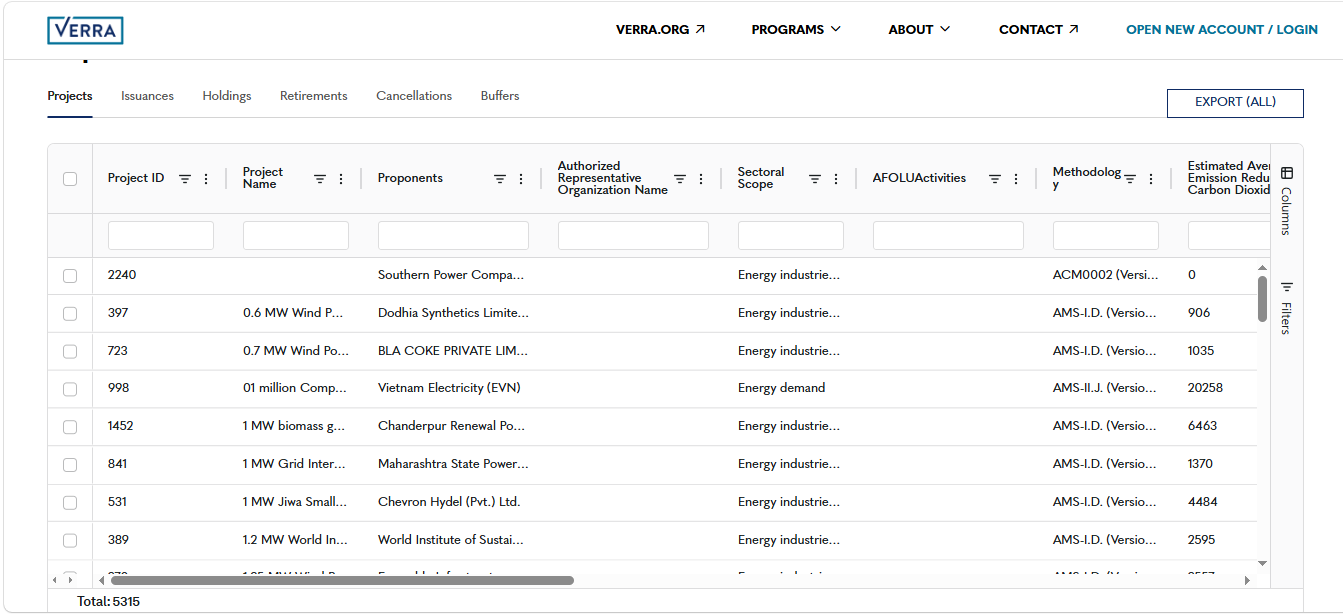
\includegraphics[width=0.9\textwidth]{image/verra_registry.png}
    \caption[Danh sách dự án thuộc chương trình VCS trên Verra Registry]%
    {Danh sách dự án thuộc chương trình VCS trên Verra Registry~\cite{verraregistry}.}
    \label{fig:verra}
\end{figure}

Ở cấp độ quốc gia, Chương trình phát triển Liên hợp quốc (UNDP) đã cung cấp một khuôn mẫu kiến trúc đáng tham khảo thông qua National Carbon Credit Registry\index{He thong dang ky@Hệ thống đăng ký (registry)!UNDP National Carbon Registry} (phiên bản 2.0). Được phát triển dưới dạng Hàng hóa công kỹ thuật số (DPG)\index{DPG (Digital Public Good)} mã nguồn mở, hệ thống này hỗ trợ các quốc gia đang phát triển xây dựng hệ thống đăng ký quốc gia phục vụ Điều~6 Thỏa thuận Paris~\cite{undp2024nationalregistry}. Về mặt kỹ thuật, dữ liệu gốc của hệ thống được ghi trong hai sổ cái: sổ cái dự án (Project ledger) và sổ cái khối tín chỉ (Credit Blocks Ledger); cơ sở dữ liệu quan hệ PostgreSQL\index{PostgreSQL} đóng vai trò cơ sở dữ liệu thứ cấp, phục vụ vận hành và truy vấn phân tích~\cite{undp2024nationalregistry}. Hệ thống được triển khai trên nền tảng đám mây AWS theo kiến trúc không máy chủ (serverless)\index{Serverless}, với các hàm AWS Lambda\index{AWS Lambda}: \texttt{national-api} xử lý các yêu cầu HTTP từ người dùng, còn \texttt{replicator} được kích hoạt bởi luồng dữ liệu Kinesis để sao chép các bản ghi từ sổ cái sang PostgreSQL~\cite{undp2024nationalregistry}.

Một điểm đáng chú ý trong thiết kế của UNDP là cách quản lý khối tín chỉ có số sê-ri liên tục (Credit Blocks)\index{Khoi tin chi@Khối tín chỉ (Credit Block)}. Khi chỉ một phần của khối tín chỉ được chuyển nhượng hoặc hủy (partial block transfer)\index{Khoi tin chi@Khối tín chỉ (Credit Block)!chuyen nhuong mot phan@chuyển nhượng một phần}, hệ thống tách dãy số sê-ri: chủ sở hữu hiện tại giữ lại phần đầu của dãy, người nhận nhận phần sau, nhờ đó vẫn truy vết được từng tín chỉ theo số sê-ri~\cite{undp2024nationalregistry}. Hệ thống cũng có chức năng tạo báo cáo theo Định dạng điện tử thỏa thuận (Agreed Electronic Format -- AEF)\index{AEF (Agreed Electronic Format)} phục vụ yêu cầu báo cáo của Điều~6.2 và hỗ trợ trao đổi dữ liệu qua tệp (ví dụ CSV)~\cite{undp2024nationalregistry}.

\subsection*{Nền tảng siêu dữ liệu phân tán: kiến trúc CAD Trust và CDOP}
\label{subsec:cadtrust}

Các hệ thống đăng ký riêng lẻ chưa liên thông với nhau, gây khó khăn cho việc đối chiếu dữ liệu tín chỉ ở quy mô toàn cầu. Để giải quyết vấn đề này, Climate Action Data Trust (CAD Trust)\index{CAD Trust} được thành lập bởi Ngân hàng Thế giới, Chính phủ Singapore và IETA, phát triển từ nền tảng Climate Warehouse của Ngân hàng Thế giới~\cite{cadtrust2025datamodel}. CAD Trust không cấp tín chỉ và không thay thế các hệ thống đăng ký hiện có; thay vào đó, nó hoạt động như một lớp siêu dữ liệu (metadata layer)\index{Lop sieu du lieu@Lớp siêu dữ liệu (metadata layer)} phi tập trung, liên kết, tổng hợp và chuẩn hóa dữ liệu từ nhiều hệ thống đăng ký (bao gồm Verra, Gold Standard\index{Gold Standard}, Global Carbon Council, v.v.)~\cite{cadtrust2025datamodel}. Hệ sinh thái dữ liệu của CAD Trust được minh họa trong \autoref{fig:cadtrust}.

\begin{figure}[htbp]
    \centering
    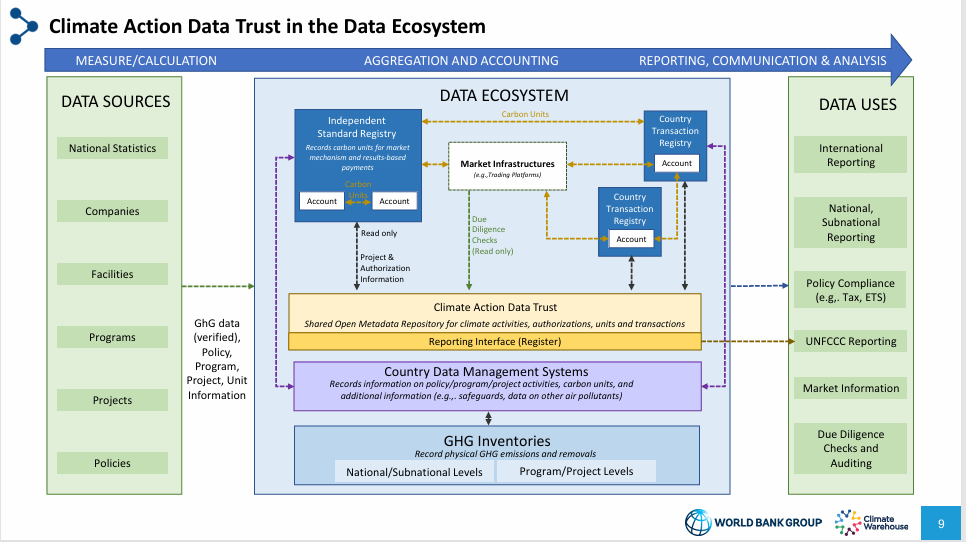
\includegraphics[width=0.9\textwidth]{image/cadtrust_ecosystem.png}
    \caption[Hệ sinh thái dữ liệu của CAD Trust]%
    {Hệ sinh thái dữ liệu của CAD Trust: nguồn dữ liệu, lớp siêu dữ liệu và các ứng dụng khai thác~\cite{cadtrust2022deepdive}.}
    \label{fig:cadtrust}
\end{figure}


CAD Trust được vận hành cùng Chia Network, dựa trên blockchain công khai Chia và thành phần Chia Data Layer\index{Chia Data Layer}. Thay vì tập trung dữ liệu vào một máy chủ duy nhất, mỗi hệ thống đăng ký tham gia chạy một nút Chia trên hạ tầng của mình và tự quản lý dữ liệu của mình. Mỗi lần cập nhật dữ liệu, mã băm mật mã\index{Ham bam mat ma@Hàm băm mật mã} của bản cập nhật được ghi lên blockchain Chia; các tệp dữ liệu được sao chép lên lưu trữ đám mây, và một cơ sở dữ liệu MySQL được dùng để phục vụ truy vấn, phân tích~\cite{cadtrust2025datamodel}. Các bên tham gia có thể tải xuống, đồng bộ và đối chiếu dữ liệu nhận được với mã băm trên blockchain để phát hiện dữ liệu bị thay đổi, mà không phải dựa vào một máy chủ trung gian duy nhất~\cite{cadtrust2025datamodel}.

Thành phần trung tâm của CAD Trust là Mô hình dữ liệu phiên bản 2.0 (Data Model Version 2.0)\index{CAD Trust!Mo hinh du lieu 2.0@Mô hình dữ liệu 2.0}, được công bố ngày 23/10/2025~\cite{cadtrust2025datamodel}. Phiên bản 1 có 9 bảng; phiên bản 2.0 giữ các bảng chung (Project, Location, Rating, Co-benefits, Estimations, Issuances, Labels, Units) và bổ sung các bảng Stakeholders, Methodologies, Programs, Validations, Verifications, Unit Labels, Project Methodologies cùng 5 bảng AEF phục vụ báo cáo theo Điều~6.2. Các hệ thống đăng ký thành viên dự kiến chuyển sang phiên bản mới trong quý I--II/2026~\cite{cadtrust2025datamodel}. Bảng~\ref{tab:cadtrust} tóm tắt các thực thể liên quan trực tiếp đến đồ án.

\begin{table}[htbp]
    \centering
    \caption{Các thực thể dữ liệu chính trong mô hình CAD Trust V2.0}
    \label{tab:cadtrust}
    \small
    \renewcommand{\arraystretch}{1.25}
    \begin{tabularx}{\textwidth}{|p{3.2cm}|X|}
        \hline
        \textbf{Thực thể dữ liệu (bảng)} & \textbf{Thuộc tính khóa và thông tin mô tả} \\
        \hline
        Project (dự án) & Thông tin định danh dự án (mã dự án trên hệ thống đăng ký gốc), chương trình, lĩnh vực, trạng thái; liên kết với các bảng Location (vị trí địa lý)\index{GIS} và Rating (xếp hạng)~\cite{cadtrust2025datamodel}. \\
        \hline
        Stakeholders (các bên liên quan) & Bảng mới của V2.0, lưu các tổ chức tham gia dự án và vai trò của họ~\cite{cadtrust2025datamodel}. \\
        \hline
        Validations, Verifications & Bảng mới của V2.0, lưu thông tin các đợt validation và verification của dự án~\cite{cadtrust2025datamodel}. \\
        \hline
        Issuances (đợt cấp) & Mỗi bản ghi là một đợt cấp tín chỉ của dự án, liên kết với Project~\cite{cadtrust2025datamodel}. \\
        \hline
        Units (đơn vị tín chỉ) & Khối tín chỉ với dãy số sê-ri, năm thực hiện giảm phát thải (Vintage Year)\index{Vintage Year}, trạng thái (Issued, Held, Retired); với tín chỉ đã hủy, lưu thêm ngày hủy và người thụ hưởng (beneficiary)~\cite{cadtrust2025datamodel}. \\
        \hline
    \end{tabularx}
\end{table}

Mô hình dữ liệu này được thiết kế để bổ sung cho Giao thức mở dữ liệu các-bon (Carbon Data Open Protocol -- CDOP)\index{CDOP (Carbon Data Open Protocol)}. CDOP là một lược đồ dữ liệu mã nguồn mở do liên minh CDOP phát triển nhằm giảm tình trạng phân mảnh định dạng dữ liệu (fragmentation) và giảm chi phí hành chính. Liên minh ra mắt tháng 3/2025, do Global Carbon Market Utility, Sylvera, RMI và S\&P Global Commodity Insights đồng chủ trì, với 37 tổ chức cam kết tham gia, trong đó có Verra, Isometric và South Pole; phiên bản 1.0 được công bố ngày 23/9/2025~\cite{cdop2025press}. CDOP V1.0 tập trung vào dữ liệu trước khi cấp tín chỉ (pre-issuance) như thông tin vị trí dự án, phương pháp luận và hồ sơ công bố, còn CAD Trust tập trung vào dữ liệu sau khi cấp (post-issuance); kết hợp lại, hai mô hình bao phủ phần lớn vòng đời dữ liệu của một tín chỉ~\cite{cadtrust2025datamodel} \cite{cdop2025press}.

% ------------------------------------------------------------
\section{Khung pháp lý thị trường các-bon tại Việt Nam và ứng dụng thực tiễn}
\label{sec:vietnam}

Một hệ thống quản lý tín chỉ các-bon được phát triển tại Việt Nam, dù ở dạng đồ án hay sản phẩm thương mại, cần tương thích với khung pháp lý quốc gia. Văn bản pháp lý chính hiện nay là Nghị định 06/2022/NĐ-CP\index{Nghi dinh 06/2022/ND-CP@Nghị định 06/2022/NĐ-CP} quy định giảm nhẹ phát thải khí nhà kính và bảo vệ tầng ô-dôn, được sửa đổi, bổ sung bởi Nghị định 119/2025/NĐ-CP, Nghị định 83/2026/NĐ-CP, 112/2026/NĐ-CP và 396/2026/NĐ-CP~\cite{vietnam2022nghidinh06}. Từ tháng 3/2025, Bộ Tài nguyên và Môi trường được hợp nhất vào Bộ Nông nghiệp và Môi trường, nên các nhiệm vụ của Bộ trong Nghị định do Bộ Nông nghiệp và Môi trường thực hiện.

Nghị định đặt ra lộ trình phát triển thị trường các-bon trong nước, bao gồm cơ chế trao đổi, bù trừ tín chỉ các-bon giữa thị trường nội địa và quốc tế~\cite{vietnam2022nghidinh06}. Các cơ sở thuộc danh mục phải kiểm kê khí nhà kính được yêu cầu kiểm kê phát thải, và Bộ Nông nghiệp và Môi trường phân bổ hạn ngạch phát thải khí nhà kính\index{Han ngach phat thai@Hạn ngạch phát thải} cho các cơ sở phát thải lớn. Một hệ thống phần mềm quản lý tại Việt Nam do đó không chỉ đơn thuần theo dõi các giao dịch tự nguyện, mà còn phải cung cấp tính năng hạch toán hạn ngạch (cap-and-trade)\index{Cap-and-trade}. Thiết kế của hệ thống cần phân biệt rõ tín chỉ tự nguyện (chẳng hạn VCUs từ Verra hoặc Gold Standard) với hạn ngạch và tín chỉ thuộc thị trường trong nước do cơ quan nhà nước quản lý, đồng thời hỗ trợ lập các báo cáo định kỳ~\cite{vietnam2022nghidinh06}.

% ------------------------------------------------------------
% ============================================================
% MỤC KHẢO SÁT SƠ BỘ HỆ THỐNG — trước mục Nhiệm vụ đồ án
% BẢN NHÁP: sinh viên đọc lại, kiểm tra nguồn và viết lại theo văn phong của mình.
% [VIẾT SAU] = phần chưa làm (phỏng vấn, câu trỏ tới mục chưa viết), đang để trong chú thích.
% Nguồn chính: Thông tư 11/2026/TT-BNNMT (đã đọc toàn văn), Nghị định 29/2026/NĐ-CP,
% Quyết định 232/QĐ-TTg, các mục 1.1–1.4 và mục 2.x (Toucan, Vaccargiu, Tsai).
% Thời gian khảo sát: khoảng tháng 9–11/2026 (các nguồn được truy cập ngày 28/9, 20/10 và 04/11/2026).
% ============================================================

\section{Khảo sát sơ bộ hệ thống}
\label{sec:khaosatsobo}

Các mục \ref{sec:dongluc}--\ref{sec:vietnam} đã trình bày bối cảnh thị trường, các tiêu chuẩn MRV, các hệ thống đăng ký quốc tế và khung pháp lý tại Việt Nam. Mục này tổng hợp các nội dung đó theo cấu trúc của một cuộc khảo sát hệ thống: xác định đơn vị và hệ thống đang vận hành, mô tả quy trình nghiệp vụ, dữ liệu và công cụ hiện có, đánh giá ưu điểm và hạn chế, từ đó rút ra nhu cầu đối với hệ thống mà đồ án xây dựng.

% ------------------------------------------------------------
\FloatBarrier
\subsection*{Giới thiệu chung}
\label{subsec:ks-gioithieu}

\subsubsection*{Lý do khảo sát}

Thị trường các-bon trong nước đang chuyển từ giai đoạn xây dựng chính sách sang giai đoạn vận hành. Đề án thành lập và phát triển thị trường các-bon tại Việt Nam theo Quyết định 232/QĐ-TTg chia lộ trình thành giai đoạn thí điểm từ năm 2025 đến hết năm 2028 và giai đoạn vận hành chính thức từ năm 2029~\cite{vietnam2025qd232}. Trong năm 2026, Thông tư 11/2026/TT-BNNMT quy định việc quản lý, vận hành Hệ thống đăng ký quốc gia về hạn ngạch phát thải khí nhà kính và tín chỉ các-bon (có hiệu lực từ ngày 30/3/2026)~\cite{vietnam2026thongtu11}, và sàn giao dịch các-bon trong nước được khai trương ngày 29/6/2026~\cite{dbnd2026santhuong}. Vì các hệ thống này mới đi vào hoạt động, trước khi xây dựng một hệ thống quản lý tín chỉ các-bon trên blockchain cần khảo sát xem các hệ thống hiện có đã đáp ứng được những gì, còn hạn chế ở đâu, để hệ thống của đồ án bổ sung đúng chỗ thay vì làm lại những chức năng đã có.

\subsubsection*{Mục tiêu khảo sát}

Cuộc khảo sát sơ bộ hướng tới các mục tiêu sau:
\begin{itemize}
    \item Xác định các bên liên quan trong vòng đời một tín chỉ các-bon (cấp, lưu ký, giao dịch, bù trừ và hủy) và vai trò của từng bên.
    \item Mô tả quy trình nghiệp vụ, dữ liệu và công cụ mà các hệ thống hiện tại đang sử dụng.
    \item Đánh giá ưu điểm, nhược điểm của hệ thống đăng ký quốc gia của Việt Nam và một số hệ thống quốc tế tiêu biểu.
    \item Rút ra nhu cầu chức năng, nhu cầu phi chức năng và định hướng giải pháp cho hệ thống mới, làm đầu vào cho phần phân tích yêu cầu ở các chương sau.
\end{itemize}
% [VIẾT SAU] Khi khôi phục Chương 3: "ở Chương~\ref{chap:thietke}" thay cho "ở các chương sau".

\subsubsection*{Phạm vi khảo sát}

Cuộc khảo sát tập trung vào giai đoạn \emph{sau khi} tín chỉ được cấp: đăng ký, định danh, chuyển quyền sở hữu, giao dịch, bù trừ và hủy tín chỉ. Khâu MRV tại thực địa (đo đạc, lập báo cáo giám sát) chỉ được xem xét ở mức đầu vào của quy trình. Về hệ thống, cuộc khảo sát gồm hai nhóm: (1) hạ tầng thị trường các-bon trong nước, gồm Hệ thống đăng ký quốc gia và hệ thống của sàn giao dịch; (2) các hệ thống quốc tế, gồm Verra Registry, UNDP National Carbon Registry, CAD Trust đã được giới thiệu ở mục \ref{sec:sodangky} và Toucan Protocol, một giao thức token hóa tín chỉ các-bon trên blockchain~\cite{toucan2025docs}. Cuộc khảo sát được thực hiện trong khoảng từ tháng 9 đến tháng 11/2026.

\subsubsection*{Đối tượng và phương pháp khảo sát}
\label{subsubsec:ks-phuongphap}

Đối tượng khảo sát là các bên liên quan trong vòng đời tín chỉ các-bon (Bảng~\ref{tab:ks-doituong}). Do chưa tiếp cận được người dùng thực tế của các hệ thống, cuộc khảo sát sơ bộ kết hợp hai phương pháp: nghiên cứu tài liệu (desk research) và quan sát các hệ thống đang vận hành. Nghiên cứu tài liệu dựa trên ba nguồn chính:
% [VIẾT SAU - PHỎNG VẤN] Câu cũ: "Trong khuôn khổ thời gian của đồ án, sinh viên chưa thực hiện được
% phỏng vấn trực tiếp với các bên này. Vì vậy cuộc khảo sát sơ bộ sử dụng phương pháp nghiên cứu tài liệu..."
% -> viết lại sau khi có kết quả phỏng vấn (bổ sung phương pháp phỏng vấn vào đây).
\begin{itemize}
    \item Văn bản pháp luật: Nghị định 06/2022/NĐ-CP và các văn bản sửa đổi, Quyết định 232/QĐ-TTg, Nghị định 29/2026/NĐ-CP và Thông tư 11/2026/TT-BNNMT. Đây là nguồn mô tả chính thức về quy trình, dữ liệu và trách nhiệm của từng bên trong hệ thống trong nước.
    \item Tài liệu kỹ thuật và giao diện công khai của các hệ thống quốc tế: trang tra cứu của Verra Registry, tài liệu của UNDP National Carbon Registry, mô hình dữ liệu CAD Trust V2.0 và tài liệu cho nhà phát triển của Toucan Protocol.
    \item Bài báo khoa học và tin tức chính thống: các nghiên cứu về ứng dụng blockchain trong quản lý tín chỉ các-bon~\cite{vaccargiu2026blockchain} \cite{tsai2024blockchain} và tin tức về sự kiện khai trương, số liệu giao dịch của sàn giao dịch các-bon trong nước.
\end{itemize}
Phương pháp quan sát gồm việc truy cập trang công khai của các hệ thống (không cần tài khoản), đọc quy trình nội bộ mà cơ quan quản lý đã ban hành và thu thập số liệu vận hành mà các đơn vị đã công bố; kết quả được trình bày ở phần Khảo sát quan sát các hệ thống thực tế. Dù vậy, kết quả khảo sát vẫn chủ yếu phản ánh quy trình \emph{theo quy định và theo tài liệu công bố}, chưa phản ánh đầy đủ khó khăn thực tế của người dùng.
% [VIẾT SAU - PHỎNG VẤN] Câu cũ: "Cột cuối của Bảng~\ref{tab:ks-doituong} ghi các thông tin dự kiến thu thập
% thêm khi có điều kiện phỏng vấn, để kiểm chứng lại các nhận định ở mục \ref{subsec:ks-danhgia}."

% [VIẾT SAU - PHỎNG VẤN] Bảng tạm bỏ cột thứ ba "Thông tin cần kiểm chứng qua phỏng vấn".
% Nội dung cột đó được giữ dưới dạng chú thích ngay dưới từng dòng; khi có kết quả phỏng vấn,
% đổi lại {|p{3.2cm}|X|X|}, thêm tiêu đề cột và điền kết quả.
\begin{table}[htbp]
    \centering
    \caption{Các bên liên quan và nguồn thông tin}
    \label{tab:ks-doituong}
    \small
    \renewcommand{\arraystretch}{1.2}
    \begin{tabularx}{\textwidth}{|p{4.2cm}|X|}
        \hline
        \textbf{Bên liên quan} & \textbf{Nguồn thông tin đã sử dụng} \\
        \hline
        Cơ quan quản lý (Cục Biến đổi khí hậu, Bộ Nông nghiệp và Môi trường) & Thông tư 11/2026/TT-BNNMT, Quyết định 232/QĐ-TTg, quy trình nội bộ thực hiện thủ tục hành chính ban hành kèm Quyết định 2935/QĐ-BNNMT~\cite{vietnam2026thongtu11} \cite{vietnam2025qd232} \cite{mae2025qd2935} \\
        % Cần hỏi: khối lượng hồ sơ xử lý thủ công, các trường hợp sai lệch khi đối soát, nhu cầu công khai dữ liệu
        \hline
        Hạ tầng sàn giao dịch (HNX, VSDC) & Nghị định 29/2026/NĐ-CP, thông tin sự kiện trên trang HNX, tin tức khai trương sàn và số liệu giao dịch do HNX công bố~\cite{vietnam2026nghidinh29} \cite{hnx2026vn2025} \cite{dbnd2026santhuong} \cite{dantri2026san3thang} \\
        % Cần hỏi: định dạng dữ liệu trao đổi với Hệ thống đăng ký quốc gia, thời gian xử lý ký gửi và thanh toán
        \hline
        Chủ dự án tạo tín chỉ & Quy trình của Verra và của Nghị định 06/2022/NĐ-CP~\cite{verra2024vcs} \cite{vietnam2022nghidinh06} \\
        % Cần hỏi: chi phí, thời gian từ khi nộp hồ sơ tới khi được cấp tín chỉ; khó khăn khi chứng minh nguồn gốc tín chỉ với bên mua
        \hline
        Đơn vị thẩm định độc lập (VVB) & ISO 14064-3, quy trình thẩm định của Verra~\cite{iso14064-3} \cite{verra2024projecthub} \\
        % Cần hỏi: cách lưu trữ và chia sẻ báo cáo thẩm định, nhu cầu ký số kết quả thẩm định
        \hline
        Doanh nghiệp mua, sử dụng tín chỉ để bù trừ & Quy định bù trừ trong Nghị định 06/2022/NĐ-CP và Thông tư 11/2026/TT-BNNMT, nghiên cứu của Tsai~\cite{vietnam2025nghidinh119} \cite{vietnam2026thongtu11} \cite{tsai2024blockchain} \\
        % Cần hỏi: cách doanh nghiệp chứng minh với khách hàng, đối tác nước ngoài rằng tín chỉ đã được hủy và không bị dùng lại
        \hline
        Người dùng công khai (nhà nghiên cứu, báo chí, tổ chức xã hội) & Trang tra cứu công khai của Verra Registry, CAD Trust~\cite{verraregistry} \cite{verra2020registryv2} \cite{cadtrust2025datamodel} \\
        % Cần hỏi: mức độ chi tiết của dữ liệu cần tra cứu (theo dự án, theo số sê-ri, theo người thụ hưởng)
        \hline
    \end{tabularx}
\end{table}

% ------------------------------------------------------------
\FloatBarrier
\subsection*{Tổng quan hệ thống hiện tại}
\label{subsec:ks-tongquan}

\subsubsection*{Giới thiệu đơn vị}

Khác với khảo sát hệ thống thông tin của một doanh nghiệp, thị trường tín chỉ các-bon không do một đơn vị duy nhất vận hành. Tại Việt Nam, đơn vị trung tâm là Bộ Nông nghiệp và Môi trường, cơ quan duy nhất có thẩm quyền cấp và quản lý mã trong nước, số sê-ri cho hạn ngạch phát thải và tín chỉ các-bon~\cite{vietnam2026thongtu11}. Trong Bộ, Cục Biến đổi khí hậu chủ trì tổ chức, quản lý và vận hành Hệ thống đăng ký quốc gia\index{He thong dang ky quoc gia@Hệ thống đăng ký quốc gia}, còn Cục Chuyển đổi số bảo đảm an toàn thông tin, hạ tầng kỹ thuật và kết nối dữ liệu của hệ thống~\cite{vietnam2026thongtu11}.

Hệ thống đăng ký quốc gia là nơi ghi nhận tập trung, thống nhất toàn bộ hạn ngạch và tín chỉ các-bon trên lãnh thổ Việt Nam. Theo Điều~4 Thông tư 11/2026/TT-BNNMT, hệ thống lưu danh sách chủ sở hữu, số lượng, mã trong nước, số sê-ri, trạng thái và lịch sử các hoạt động; mọi nghiệp vụ được thực hiện dưới dạng giao dịch điện tử~\cite{vietnam2026thongtu11}. Bên cạnh hệ thống đăng ký, sàn giao dịch các-bon trong nước\index{San giao dich carbon@Sàn giao dịch các-bon} được tổ chức theo Nghị định 29/2026/NĐ-CP với Sở Giao dịch Chứng khoán Hà Nội (HNX)\index{HNX} tổ chức giao dịch và Tổng công ty Lưu ký và Bù trừ Chứng khoán Việt Nam (VSDC)\index{VSDC} phụ trách lưu ký, chuyển quyền sở hữu và thanh toán~\cite{vietnam2026nghidinh29}.

Sàn được khai trương ngày 29/6/2026. Hàng hóa đầu tiên được đưa lên sàn là hạn ngạch phát thải mã VN2025 với tổng khối lượng 511.473.846~tCO$_2$e cho giai đoạn tuân thủ 2025--2026; ngày giao dịch cuối cùng của mã này là 24/12/2027~\cite{hnx2026vn2025}. Theo Quyết định 263/QĐ-TTg, tổng hạn ngạch này gồm 243.082.392~tCO$_2$e cho năm 2025 và 268.391.454~tCO$_2$e cho năm 2026, phân bổ cho 110 cơ sở thuộc ba lĩnh vực: 34 cơ sở nhiệt điện, 25 cơ sở sản xuất sắt thép và 51 cơ sở sản xuất xi măng~\cite{vietnam2026qd263}. Trong giai đoạn thí điểm đến hết năm 2028, HNX, VSDC và Sở Giao dịch Chứng khoán Việt Nam (VNX) không thu phí dịch vụ trên sàn~\cite{vietnam2026nghidinh29}.
% Số liệu VN2025 đã được sinh viên đối chiếu với thông tin sự kiện trên trang HNX (04/11/2026).
% 110 cơ sở (34 + 25 + 51) và hạn ngạch từng năm: bản ký số QĐ 263/QĐ-TTg ngày 09/02/2026 (đã đọc 04/11/2026).

Ngoài hệ thống trong nước, Việt Nam đã tham gia thị trường các-bon quốc tế qua các cơ chế chi trả dựa trên kết quả. Ngày 22/10/2020, Việt Nam ký Thỏa thuận chi trả giảm phát thải (ERPA)\index{ERPA} với Ngân hàng Thế giới trong khuôn khổ Quỹ đối tác các-bon lâm nghiệp (FCPF)\index{FCPF} cho lượng giảm phát thải từ rừng tại sáu tỉnh Bắc Trung Bộ trong giai đoạn 2018--2024~\cite{worldbank2020erpa}. Tháng 3/2024, Việt Nam nhận khoản thanh toán 51,5 triệu USD, với đơn giá 5~USD/tấn, cho 10,3 triệu tấn CO$_2$ giảm phát thải trong khoảng từ ngày 01/02/2018 đến ngày 31/12/2019~\cite{baochinhphu2024erpa}; theo Nghị quyết 261/NQ-CP ngày 29/8/2025, Việt Nam chuyển nhượng bổ sung 1 triệu tấn CO$_2$ của giai đoạn 2018--2019~\cite{vietnamfinance2025erpa}. Nhiều dự án tại Việt Nam cũng đăng ký trên các chương trình tự nguyện như VCS của Verra (mục \ref{sec:mrv}). Vì vậy, các hệ thống quốc tế ở mục \ref{sec:sodangky} cũng là đối tượng khảo sát của mục này.

\subsubsection*{Mô hình tổ chức}

\HinhMoHinhToChuc

Mô hình tổ chức của thị trường các-bon trong nước được tổng hợp trong \autoref{fig:mohinhtochuc}. Có thể chia các bên thành ba nhóm:
\begin{itemize}
    \item Nhóm tạo tín chỉ: chủ dự án lập hồ sơ và thực hiện giám sát; đơn vị thẩm định độc lập thẩm định hồ sơ và kết quả giảm phát thải; cơ quan có thẩm quyền quyết định cấp tín chỉ. Theo Nghị định 396/2026/NĐ-CP, có hiệu lực từ ngày 12/12/2026, Chủ tịch Ủy ban nhân dân cấp tỉnh nơi tiếp nhận hồ sơ quyết định cấp tín chỉ theo cơ chế trong nước; trước ngày này, thẩm quyền thuộc bộ quản lý lĩnh vực (hoặc Bộ Nông nghiệp và Môi trường)~\cite{vietnam2026nghidinh396}. Với tín chỉ theo Điều~6.2, Điều~6.4 Thỏa thuận Paris, thông báo cấp đến từ cơ quan, tổ chức cấp tín chỉ của cơ chế quốc tế tương ứng~\cite{vietnam2026thongtu11}.
    \item Nhóm quản lý dữ liệu gốc: Bộ Nông nghiệp và Môi trường vận hành Hệ thống đăng ký quốc gia. Dữ liệu trên hệ thống này là dữ liệu gốc để đối chiếu khi các hệ thống có sai lệch, trừ dữ liệu về lưu ký, giao dịch và thanh toán~\cite{vietnam2026thongtu11}.
    \item Nhóm hạ tầng giao dịch: HNX vận hành hệ thống giao dịch, VSDC vận hành hệ thống lưu ký và thanh toán, ngân hàng thanh toán xử lý dòng tiền, VNX thực hiện chế độ báo cáo về giao dịch cho Bộ Nông nghiệp và Môi trường~\cite{vietnam2026nghidinh29} \cite{vietnam2026thongtu11}.
\end{itemize}
Chủ tài khoản là các cơ sở được phân bổ hạn ngạch và các tổ chức có chương trình, dự án tín chỉ; mỗi tổ chức chỉ được cấp một tài khoản đăng ký, gắn với mã số thuế~\cite{vietnam2026thongtu11}.

\subsubsection*{Chức năng và nhiệm vụ}

Theo Điều~26 Thông tư 11/2026/TT-BNNMT, Cục Biến đổi khí hậu có các nhiệm vụ chính: đăng ký, hủy đăng ký, cấp và quản lý mã trong nước, số sê-ri; mở, phong tỏa, giải tỏa và đóng tài khoản đăng ký; tiếp nhận và xử lý đề nghị nghiệp vụ của chủ tài khoản; chủ trì đối soát và chia sẻ dữ liệu; công bố thông tin định kỳ; xây dựng tài liệu hướng dẫn và đào tạo người dùng~\cite{vietnam2026thongtu11}. Cục Chuyển đổi số chịu trách nhiệm an toàn, an ninh thông tin, phương án sao lưu, dự phòng và giải pháp kết nối dữ liệu với hệ thống của HNX, VSDC và các nền tảng số quốc gia~\cite{vietnam2026thongtu11}. HNX và VSDC phối hợp với Cục Biến đổi khí hậu theo Biên bản phối hợp giữa các bên, gửi báo cáo đối soát cuối ngày, báo cáo định kỳ và báo cáo sự cố trong vòng 24 giờ~\cite{vietnam2026thongtu11}.

\subsubsection*{Các hệ thống và phần mềm đang sử dụng}

Bảng~\ref{tab:ks-hethong} liệt kê các hệ thống đang được sử dụng trong vòng đời tín chỉ các-bon mà đồ án khảo sát. Ba hệ thống đầu thuộc hạ tầng trong nước; các hệ thống còn lại là hệ thống quốc tế, trong đó Verra Registry, UNDP National Carbon Registry và CAD Trust đã được mô tả ở mục \ref{sec:sodangky}.

\begin{table}[htbp]
    \centering
    \caption{Các hệ thống đang sử dụng trong vòng đời tín chỉ các-bon}
    \label{tab:ks-hethong}
    \small
    \renewcommand{\arraystretch}{1.2}
    \begin{tabularx}{\textwidth}{|p{3.1cm}|p{2.6cm}|X|p{2.6cm}|}
        \hline
        \textbf{Hệ thống} & \textbf{Đơn vị vận hành} & \textbf{Chức năng chính} & \textbf{Nền tảng} \\
        \hline
        Hệ thống đăng ký quốc gia & Bộ NN\&MT (Cục Biến đổi khí hậu) & Tài khoản đăng ký, cấp mã trong nước và số sê-ri, ký gửi, bù trừ, nộp trả, hủy~\cite{vietnam2026thongtu11} & Cơ sở dữ liệu tập trung, xác thực qua Cổng dịch vụ công quốc gia \\
        \hline
        Hệ thống giao dịch các-bon & HNX & Khớp lệnh, công bố kết quả giao dịch~\cite{vietnam2026nghidinh29} & Tập trung \\
        \hline
        Hệ thống lưu ký và thanh toán giao dịch các-bon & VSDC & Tài khoản lưu ký, chuyển quyền sở hữu, thanh toán, đối soát cuối ngày~\cite{vietnam2026nghidinh29} \cite{vietnam2026thongtu11} & Tập trung \\
        \hline
        Verra Registry và Verra Project Hub & Verra & Đăng ký dự án, cấp VCU có số sê-ri, hủy tín chỉ, tra cứu công khai~\cite{verra2024vcs} \cite{verra2024projecthub} & Tập trung, giao diện web \\
        \hline
        UNDP National Carbon Registry & Các quốc gia tự triển khai & Hệ thống đăng ký quốc gia mã nguồn mở phục vụ Điều~6, báo cáo AEF~\cite{undp2024nationalregistry} & Sổ cái và PostgreSQL trên AWS \\
        \hline
        CAD Trust & CAD Trust, Chia Network & Lớp siêu dữ liệu liên thông các hệ thống đăng ký~\cite{cadtrust2025datamodel} & Blockchain Chia, MySQL \\
        \hline
        Toucan Protocol & Toucan & Token hóa tín chỉ đã cấp, pool ERC-20, hủy tín chỉ on-chain~\cite{toucan2025docs} & Polygon, Celo (EVM) \\
        \hline
    \end{tabularx}
\end{table}

% ------------------------------------------------------------
\FloatBarrier
\subsection*{Khảo sát hiện trạng}
\label{subsec:ks-hientrang}

\subsubsection*{Quy trình nghiệp vụ}

Từ Thông tư 11/2026/TT-BNNMT, vòng đời của một tín chỉ các-bon trên hệ thống trong nước có thể mô tả qua ba nhóm quy trình.

a) Đăng ký tín chỉ. Sau khi chủ dự án hoàn thành hồ sơ, thẩm định và được bộ quản lý lĩnh vực hoặc Bộ Nông nghiệp và Môi trường quyết định cấp tín chỉ, trong thời hạn 05 ngày làm việc Bộ Nông nghiệp và Môi trường hoàn thành việc đăng ký tín chỉ trên Hệ thống đăng ký quốc gia. Thông tin đăng ký gồm tên chương trình, dự án, tên cơ chế trao đổi, bù trừ, tổng số lượng tín chỉ và mã trong nước; thông tin chủ sở hữu gồm tên tổ chức, mã số thuế, số lượng và số sê-ri tương ứng. Trong ngày đăng ký, Bộ gửi thông tin cho chủ sở hữu và gửi mã trong nước cho HNX, VSDC qua hình thức điện tử~\cite{vietnam2026thongtu11}.

b) Ký gửi và giao dịch. Chủ tài khoản muốn giao dịch phải ký gửi tín chỉ sang hệ thống lưu ký:
\begin{enumerate}
    \item Chủ tài khoản thông báo số lượng cần ký gửi kèm thông tin tài khoản lưu ký; hệ thống chuyển số lượng này từ tiểu khoản Đăng ký chung sang tiểu khoản Chờ ký gửi, hoặc từ chối nếu số dư không đủ.
    \item Cuối mỗi ngày làm việc, Bộ Nông nghiệp và Môi trường tổng hợp danh sách đề nghị ký gửi và gửi cho VSDC.
    \item Trong thời hạn 01 ngày làm việc, VSDC xác nhận hoặc từ chối; khi được xác nhận, số lượng được chuyển sang tiểu khoản Số dư giao dịch.
    \item Giao dịch được khớp trên hệ thống của HNX; HNX chuyển kết quả cho VSDC để chuyển quyền sở hữu và thanh toán qua ngân hàng thanh toán.
\end{enumerate}
Các bước trên được lấy từ Điều~14 Thông tư 11/2026/TT-BNNMT và Nghị định 29/2026/NĐ-CP~\cite{vietnam2026thongtu11} \cite{vietnam2026nghidinh29}. Cuối mỗi ngày làm việc, VSDC gửi báo cáo kết quả thanh toán và số dư ký gửi để Bộ đối soát với dữ liệu trên Hệ thống đăng ký quốc gia (Điều~23)~\cite{vietnam2026thongtu11}.

c) Bù trừ và hủy tín chỉ. Tín chỉ bị hủy đăng ký trong ba trường hợp: được dùng để bù trừ phát thải, được chủ tài khoản hủy tự nguyện, hoặc bị thu hồi theo quyết định của cơ quan có thẩm quyền~\cite{vietnam2026thongtu11}. Khi bù trừ, tín chỉ được chuyển từ tiểu khoản Đăng ký chung sang tiểu khoản Bù trừ, sau đó Bộ tăng lượng tương ứng trên tiểu khoản Nộp trả và hủy đăng ký số tín chỉ đã dùng. Khoản 16 Điều 1 Nghị định 119/2025/NĐ-CP đã sửa đổi toàn bộ Điều 19 Nghị định 06/2022/NĐ-CP về trao đổi, vay mượn, nộp trả, chuyển giao và bù trừ. Theo Điều 19 mới, cơ sở chỉ được dùng tín chỉ để bù trừ không quá 30\% lượng hạn ngạch được phân bổ (điểm a khoản 8); đến hết năm 2030, cơ sở có thể vay mượn hạn ngạch của giai đoạn kế tiếp nhưng không quá 15\% lượng hạn ngạch đã được phân bổ, và hạn ngạch vay mượn không được dùng để trao đổi (điểm a khoản 6)~\cite{vietnam2025nghidinh119}. Khi hủy tự nguyện, chủ tài khoản nộp đơn theo Mẫu số 01 (trực tiếp, qua bưu chính hoặc trực tuyến trên Cổng dịch vụ công quốc gia); trong 02 ngày làm việc, Bộ thực hiện hủy và gửi thông báo xác nhận theo Mẫu số 02~\cite{vietnam2026thongtu11}. Việc hủy bao gồm hủy cả số lượng và số sê-ri tương ứng; khi toàn bộ tín chỉ của một mã trong nước đã bị hủy thì mã đó cũng bị hủy và không được cấp lại~\cite{vietnam2026thongtu11}.
% [ĐÃ KIỂM TRA 04/11/2026] Tỷ lệ 30% / 15% KHÔNG có trong bản gốc NĐ 06/2022 (Điều 19 cũ khác hẳn);
% chúng nằm trong Điều 19 mới do khoản 16 Điều 1 NĐ 119/2025 thay thế (hiệu lực 01/8/2025).
% Bản chính thức (Cổng TTĐT Chính phủ): https://datafiles.chinhphu.vn/cpp/files/vbpq/2025/6/119-nd.signed.pdf
%   tr. 12: "16. Sửa đổi Điều 19 như sau"; tr. 13: khoản 6 điểm a (15%); tr. 14: khoản 8 điểm a (30%).
% Các nghị định sửa đổi sau KHÔNG đụng tới Điều 19:
%   NĐ 83/2026: chỉ sửa Điều 24, 26, Phụ lục VI (ô-dôn) - https://datafiles.chinhphu.vn/cpp/files/vbpq/2026/3/83-ndcp.signed.pdf
%   NĐ 112/2026: Điều 32 khoản 2 (tr. 27) chỉ bãi bỏ khoản 2, 4, 5, 6 Điều 20a - https://datafiles.chinhphu.vn/cpp/files/vbpq/2026/4/112-ndcp.signed.pdf
%   NĐ 396/2026: chỉ sửa khoản 2 Điều 18, Điều 20, 20a, Phụ lục V - https://datafiles.chinhphu.vn/cpp/files/vbpq/2026/10/396_2026_nd-cp_26102026_3-signed.signed.pdf

Với các hệ thống quốc tế, quy trình có cấu trúc tương tự: Verra Registry quản lý mở tài khoản, yêu cầu phát hành, tạo số sê-ri và hủy tín chỉ~\cite{verra2024vcs}; Toucan Protocol thêm các bước token hóa, nạp pool và hủy trên blockchain~\cite{toucan2025docs}.

\subsubsection*{Các đối tượng tham gia}

Bảng~\ref{tab:ks-tacnhan} tổng hợp các đối tượng tham gia và hệ thống mà mỗi đối tượng đang sử dụng. Các đối tượng này là cơ sở để xác định tác nhân của hệ thống mới.
% [VIẾT SAU] Khi viết xong mục Các tác nhân (Chương 3), thêm lại: "... ở mục \ref{subsec:tacnhan}."

\begin{table}[htbp]
    \centering
    \caption{Các đối tượng tham gia vòng đời tín chỉ các-bon}
    \label{tab:ks-tacnhan}
    \small
    \renewcommand{\arraystretch}{1.2}
    \begin{tabularx}{\textwidth}{|p{3.3cm}|X|p{3.6cm}|}
        \hline
        \textbf{Đối tượng} & \textbf{Vai trò} & \textbf{Hệ thống sử dụng} \\
        \hline
        Chủ dự án & Lập hồ sơ dự án, thực hiện giám sát, nhận và sở hữu tín chỉ được cấp & Hệ thống đăng ký quốc gia; Verra Registry (với tín chỉ tự nguyện) \\
        \hline
        Đơn vị thẩm định độc lập (VVB) & Thẩm định hồ sơ dự án và kết quả giảm phát thải theo ISO 14064-3~\cite{iso14064-3} & Nộp báo cáo cho chương trình hoặc cơ quan cấp tín chỉ \\
        \hline
        Cơ quan quản lý & Quyết định cấp tín chỉ, cấp mã và số sê-ri, quản lý tài khoản, đối soát, công bố thông tin & Hệ thống đăng ký quốc gia \\
        \hline
        Cơ sở được phân bổ hạn ngạch & Mua tín chỉ, dùng tín chỉ để bù trừ, nộp trả hạn ngạch & Hệ thống đăng ký quốc gia, tài khoản lưu ký và giao dịch \\
        \hline
        Tổ chức hạ tầng (HNX, VSDC, ngân hàng) & Tổ chức giao dịch, lưu ký, thanh toán, báo cáo & Hệ thống giao dịch, hệ thống lưu ký và thanh toán \\
        \hline
        Người dùng công khai & Tra cứu thông tin dự án, tín chỉ đã cấp và đã hủy & Thông tin công bố trên Hệ thống đăng ký quốc gia; trang tra cứu Verra Registry \\
        \hline
    \end{tabularx}
\end{table}

\subsubsection*{Dữ liệu và tài liệu}

Dữ liệu cốt lõi trong hệ thống trong nước là mã trong nước\index{Ma trong nuoc@Mã trong nước} và số sê-ri. Mã trong nước của hạn ngạch gồm 6 ký tự theo cấu trúc VN[năm phân bổ], ví dụ VN2025. Mã trong nước của tín chỉ gồm 9 ký tự theo cấu trúc [mã cơ chế, 3 ký tự][mã dự án, 4 ký tự][2 số cuối của năm mà lượng giảm phát thải được xác nhận]. Số sê-ri được tạo bằng cách nối mã trong nước với một dải 10 chữ số, là số thứ tự của từng đơn vị trong tổng số lượng được cấp; như vậy mỗi tấn CO$_2$e có một số sê-ri riêng~\cite{vietnam2026thongtu11}. Cách định danh theo lô và dải số sê-ri này tương tự cách Verra và UNDP quản lý khối tín chỉ (mục \ref{sec:sodangky}).

Mỗi tài khoản đăng ký gồm 8 tiểu khoản\index{Tieu khoan@Tiểu khoản} chức năng theo Điều~7 Thông tư 11/2026/TT-BNNMT, tương ứng với các trạng thái mà một đơn vị hạn ngạch hoặc tín chỉ có thể đi qua (Bảng~\ref{tab:ks-tieukhoan}). Khi chuyển trạng thái, số lượng được chuyển giữa các tiểu khoản; các nghiệp vụ ký gửi, chuyển quyền sở hữu, chuyển giao, vay mượn chỉ được thực hiện với số lượng đang nằm ở tiểu khoản Đăng ký chung~\cite{vietnam2026thongtu11}.

\begin{table}[htbp]
    \centering
    \caption{Các tiểu khoản của tài khoản đăng ký theo Thông tư 11/2026/TT-BNNMT}
    \label{tab:ks-tieukhoan}
    \small
    \renewcommand{\arraystretch}{1.2}
    \begin{tabularx}{\textwidth}{|p{3.2cm}|X|}
        \hline
        \textbf{Tiểu khoản} & \textbf{Nội dung ghi nhận~\cite{vietnam2026thongtu11}} \\
        \hline
        Đăng ký chung & Hạn ngạch, tín chỉ thuộc sở hữu hợp pháp của chủ tài khoản, chưa đưa vào giao dịch hay nghiệp vụ khác \\
        \hline
        Số dư giao dịch & Hạn ngạch, tín chỉ đã ký gửi tại VSDC \\
        \hline
        Chuyển giao & Hạn ngạch chuyển từ giai đoạn hiện tại sang giai đoạn kế tiếp \\
        \hline
        Vay mượn & Hạn ngạch của giai đoạn kế tiếp được vay để dùng cho giai đoạn hiện tại \\
        \hline
        Bù trừ & Tín chỉ được dùng để bù trừ phát thải \\
        \hline
        Nộp trả & Hạn ngạch được chủ tài khoản nộp trả \\
        \hline
        Chờ ký gửi & Hạn ngạch, tín chỉ đã đề nghị ký gửi, đang chờ VSDC xác nhận \\
        \hline
        Phong tỏa & Hạn ngạch, tín chỉ bị phong tỏa theo yêu cầu của cơ quan có thẩm quyền \\
        \hline
    \end{tabularx}
\end{table}

Ngoài dữ liệu trên hệ thống đăng ký, quy trình còn sử dụng nhiều tài liệu dạng tệp: hồ sơ thiết kế dự án (PDD), báo cáo giám sát, báo cáo thẩm định của VVB, các biểu mẫu đề nghị và thông báo (ví dụ Mẫu số 01, Mẫu số 02 của Thông tư 11/2026/TT-BNNMT). Về công bố thông tin, Bộ Nông nghiệp và Môi trường công bố hằng tháng (chậm nhất ngày 20 tháng sau) danh sách dự án đã đăng ký và tổng số lượng hạn ngạch, tín chỉ đăng ký mới, hủy đăng ký; công bố hằng năm và hai năm một lần các số liệu tổng hợp; và công bố trong vòng 72 giờ việc cấp, hủy mã trong nước và số sê-ri~\cite{vietnam2026thongtu11}. Thông tin truy cập và thông tin giao dịch của các tổ chức tham gia phải được bảo mật~\cite{vietnam2026thongtu11}.

\subsubsection*{Công cụ hỗ trợ}

Các công cụ hỗ trợ chính của hệ thống trong nước gồm:
\begin{itemize}
    \item Định danh điện tử: mọi yêu cầu nghiệp vụ từ tài khoản đăng ký phải được xác thực qua nền tảng định danh và xác thực điện tử của Cổng dịch vụ công quốc gia; giao dịch đã xác thực có giá trị pháp lý như văn bản có chữ ký của người đại diện hợp pháp~\cite{vietnam2026thongtu11}.
    \item Cơ chế tạo và duyệt giao dịch: mỗi giao dịch nghiệp vụ do một người tạo và một người khác duyệt; chủ tài khoản tự phân công nhân sự cho hai vai trò này~\cite{vietnam2026thongtu11}.
    \item Kết nối dữ liệu giữa các hệ thống: dữ liệu giữa Hệ thống đăng ký quốc gia, hệ thống của HNX và VSDC được trao đổi qua kênh truyền dẫn riêng hoặc API được mã hóa; định dạng thông điệp được quy định trong tài liệu kỹ thuật và biên bản phối hợp giữa các bên~\cite{vietnam2026thongtu11}.
    \item Đối soát cuối ngày: báo cáo của VSDC được dùng để đối chiếu với dữ liệu trên hệ thống đăng ký~\cite{vietnam2026thongtu11}.
\end{itemize}
Ở phía quốc tế, Verra Project Hub cung cấp biểu mẫu số và các phương pháp luận được số hóa để nộp, xét duyệt hồ sơ~\cite{verra2024projecthub}; CAD Trust cung cấp mô hình dữ liệu chung và cơ chế đối chiếu mã băm trên blockchain~\cite{cadtrust2025datamodel}. Ở khâu MRV, nhiều quy trình vẫn dựa vào chuyên gia tư vấn, kiểm toán thủ công và báo cáo giấy theo chu kỳ dài~\cite{tsai2024blockchain}.

% ------------------------------------------------------------
\FloatBarrier
\subsection*{Khảo sát quan sát các hệ thống thực tế}
\label{subsec:ks-quansat}

Để kiểm tra lại các nhận định rút ra từ văn bản, đồ án quan sát trực tiếp một số hệ thống đang vận hành theo ba cách: truy cập trang công khai của hệ thống bằng trình duyệt, không đăng nhập, và ghi lại các thao tác tra cứu được; đọc quy trình nội bộ mà cơ quan quản lý đã ban hành cho các thủ tục hành chính liên quan; thu thập số liệu vận hành mà các đơn vị đã công bố. Bảng~\ref{tab:ks-quansat} tóm tắt kết quả quan sát các hệ thống trong nước, Bảng~\ref{tab:ks-quansat-qt} tóm tắt kết quả quan sát các hệ thống quốc tế. Hình~\ref{fig:ks-dvc-taikhoan} đến Hình~\ref{fig:ks-toucan} là ảnh chụp màn hình các trang công khai được quan sát, tất cả được truy cập ngày 04/11/2026.

\begin{table}[htbp]
    \centering
    \caption{Kết quả quan sát các hệ thống trong nước}
    \label{tab:ks-quansat}
    \small
    \renewcommand{\arraystretch}{1.2}
    \begin{tabularx}{\textwidth}{|>{\raggedright\arraybackslash}p{2.6cm}|>{\raggedright\arraybackslash}p{3.4cm}|X|}
        \hline
        \textbf{Hệ thống} & \textbf{Thao tác, nguồn quan sát} & \textbf{Kết quả ghi nhận} \\
        \hline
        Hệ thống đăng ký quốc gia: đăng ký tài khoản & Đọc trang thủ tục mã 1.014129 (Hình~\ref{fig:ks-dvc-taikhoan}) và quy trình nội bộ của thủ tục & Hồ sơ gồm tài liệu của dự án đã đăng ký theo cơ chế, phương thức liên lạc của dự án và đơn đề nghị theo mẫu Phụ lục 12.1 thuộc Phụ lục XII ban hành kèm theo Nghị quyết 17/2026/NQ-CP ngày 29/4/2026 của Chính phủ; nộp trực tiếp, trực tuyến hoặc qua bưu chính, cùng thời hạn 05 ngày làm việc; Cục Biến đổi khí hậu thực hiện~\cite{mae2026tthc1014129}. Hồ sơ đi qua chuyên viên, lãnh đạo phòng, lãnh đạo Cục và lãnh đạo Bộ duyệt~\cite{mae2025qd2935}. Từ ngày 12/12/2026, một số trường hợp do Chủ tịch Ủy ban nhân dân cấp tỉnh cấp tài khoản, thời hạn vẫn là 05 ngày làm việc~\cite{vietnam2026nghidinh396} \\
        \hline
        Hệ thống đăng ký quốc gia: cấp tín chỉ theo cơ chế trong nước & Đọc Nghị định 396/2026/NĐ-CP, trang thủ tục mã 1.014133 (Hình~\ref{fig:ks-dvc-tinchi}) và quy trình nội bộ của thủ tục & Quy trình hiện hành, từ ngày 12/12/2026: Chủ tịch Ủy ban nhân dân cấp tỉnh nơi tiếp nhận hồ sơ quyết định cấp, qua bốn bước 03, 03, 10 và 10 ngày làm việc, tổng cộng 26 ngày làm việc~\cite{vietnam2026nghidinh396}. Quy trình trước đó, vẫn hiển thị trên trang thủ tục ngày 04/11/2026: hồ sơ nộp tới bộ quản lý lĩnh vực (Bộ NN\&MT, Bộ Công Thương hoặc Bộ Xây dựng); kiểm tra 03 ngày làm việc, hồ sơ chưa hợp lệ phải bổ sung hoặc nộp lại; lấy ý kiến 03 ngày làm việc và 15 ngày; quyết định trong 15 ngày; tổng 06 ngày làm việc và 30 ngày~\cite{mae2026tthc1014133} \cite{mae2025qd2935} \\
        \hline
        Sàn giao dịch các-bon (HNX, VSDC): quy trình một giao dịch & Đọc hướng dẫn quy trình giao dịch do cơ quan báo chí của Bộ NN\&MT đăng ngày 01/7/2026 & Doanh nghiệp phải ký gửi trên Hệ thống đăng ký quốc gia, mở tài khoản tại thành viên giao dịch (công ty chứng khoán) và đặt lệnh qua thành viên; mỗi tổ chức chỉ dùng một tài khoản giao dịch các-bon; thanh toán tức thì khi bên mua đủ tiền và bên bán đủ hạn ngạch trên tài khoản lưu ký~\cite{nnmt2026quytrinh} \\
        \hline
        Sàn giao dịch các-bon (HNX): số liệu giao dịch & Theo dõi số liệu mã VN2025 trên trang của HNX từ ngày 29/6 đến ngày 04/11/2026 (Hình~\ref{fig:ks-hnx} và Hình~\ref{fig:ks-hnx-chitiet}) & Chỉ có giao dịch trong tháng 6 và tháng 9/2026, toàn bộ là hạn ngạch~\cite{hnx2026sanphamcacbon}; giá trong 52 tuần từ 130.000 đến 136.000 đồng/tCO$_2$e~\cite{hnx2026ketquagd}. VN2025 là mã duy nhất, tổng hạn ngạch phân bổ 511.473.846, giao dịch đến ngày 24/12/2027~\cite{hnx2026danhmuchanngach}. Theo số liệu HNX đến ngày 28/9/2026, phiên khai trương có 6 giao dịch với 1.210 hạn ngạch, giao dịch thứ 7 ngày 15/9 có 100 hạn ngạch; lũy kế 1.310 hạn ngạch, khoảng 174,8 triệu đồng, khoảng 0,00026\% tổng hạn ngạch~\cite{dantri2026san3thang} \\
        \hline
    \end{tabularx}
\end{table}

\begin{table}[htbp]
    \centering
    \caption{Kết quả quan sát các hệ thống quốc tế}
    \label{tab:ks-quansat-qt}
    \small
    \renewcommand{\arraystretch}{1.2}
    \begin{tabularx}{\textwidth}{|>{\raggedright\arraybackslash}p{2.6cm}|>{\raggedright\arraybackslash}p{3.4cm}|X|}
        \hline
        \textbf{Hệ thống} & \textbf{Thao tác, nguồn quan sát} & \textbf{Kết quả ghi nhận} \\
        \hline
        Verra Registry (trang công khai) & Truy cập \url{https://registry.verra.org} không đăng nhập; xem trang chủ và báo cáo Retirements trong mục Reports (Hình~\ref{fig:ks-verra}) & Ai cũng tra cứu được thông tin dự án và tín chỉ, nhưng phải có tài khoản Verra Registry đang hoạt động mới được đăng ký dự án hoặc yêu cầu phát hành, chuyển nhượng, hủy tín chỉ~\cite{verraregistryhome}. Báo cáo Retirements liệt kê từng lô tín chỉ đã hủy với ngày hủy, mã và tên dự án, lĩnh vực, phương pháp luận, nhãn bổ sung (ví dụ CORSIA), năm giảm phát thải (vintage) và số sê-ri; người xem có thể lọc theo từng cột và xuất toàn bộ dữ liệu. Tám dòng đầu của báo cáo đều là các lô được hủy ngày 04/11/2026, thuộc năm dự án khác nhau~\cite{verra2026retirements}. Lý do hủy và chủ sở hữu thụ hưởng là trường tùy chọn, không hiển thị nếu chủ tài khoản chọn giữ riêng tư~\cite{verraregistry} \cite{verra2020registryv2} \\
        % [VIẾT SAU - SỐ LIỆU] Lọc cột Retirement Date = 04/11/2026 trên báo cáo Retirements, ghi tổng số lô
        % (dòng) được hủy trong ngày rồi thay câu "Tám dòng đầu ..." bằng con số này.
        \hline
        CAD Trust (Public Data Dashboard) & Truy cập trang Public Data Dashboard không đăng nhập; chọn khu vực, quốc gia và khoảng thời gian trên bản đồ (Hình~\ref{fig:ks-cadtrust}) & Trang công khai hiển thị số liệu tổng hợp theo khu vực và quốc gia: số dự án đang hoạt động, tổng lượng giảm phát thải, lượng giảm phát thải ước tính hằng năm và cơ cấu theo lĩnh vực; ô Registry cho biết dữ liệu được chọn đã có trong các hệ thống đăng ký hay chưa~\cite{cadtrust2026dashboard}. Trong lần quan sát, đồ án không tìm thấy trang chi tiết của từng dự án khi không đăng nhập \\
        % [VIẾT SAU - ẢNH CHỤP] Chọn Southeast Asia -> Viet Nam trên dashboard, chụp lại và ghi số dự án,
        % lượng giảm phát thải, nội dung ô Registry của Việt Nam vào ô trên; nếu Việt Nam không có dữ liệu thì
        % ghi rõ điều đó (cũng là một phát hiện). Thay ảnh ở Hình fig:ks-cadtrust.
        \hline
        Toucan Protocol (ứng dụng web) & Truy cập \url{https://app.toucan.earth}, mục Explorer, mở trang một dự án (Hình~\ref{fig:ks-toucan}) & Trang dự án Wakefield Biochar Facility 2 ghi mã dự án PUR-244045, tiêu chuẩn gốc là Puro, phương pháp luận biochar, loại tín chỉ hấp thụ (removal), trạng thái đang hoạt động và cho biết tín chỉ của dự án đã nằm trong pool CHAR; trang có thêm tab tài liệu của dự án~\cite{toucan2026wakefield}. Dự án được quan sát là tín chỉ do Puro cấp rồi mới được token hóa, và trang giữ mã dự án của Puro \\
        \hline
    \end{tabularx}
\end{table}

\begin{figure}[htbp]
    \centering
    \begin{subfigure}{\textwidth}
        \centering
        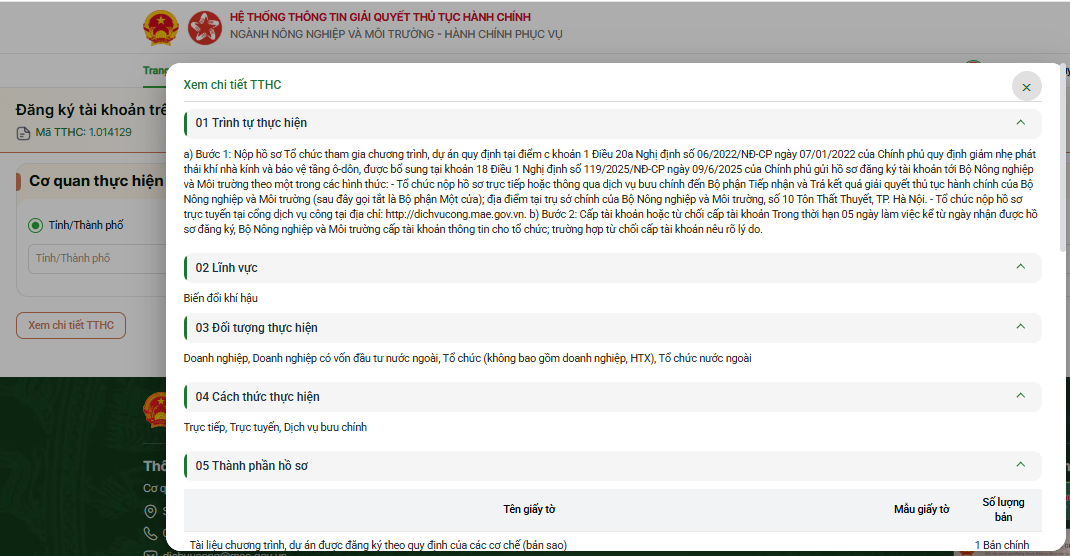
\includegraphics[width=0.8\textwidth]{image/dvc_1014129_trinh_tu.png}
        \caption{Trình tự thực hiện}
    \end{subfigure}

    \vspace{0.3cm}
    \begin{subfigure}{\textwidth}
        \centering
        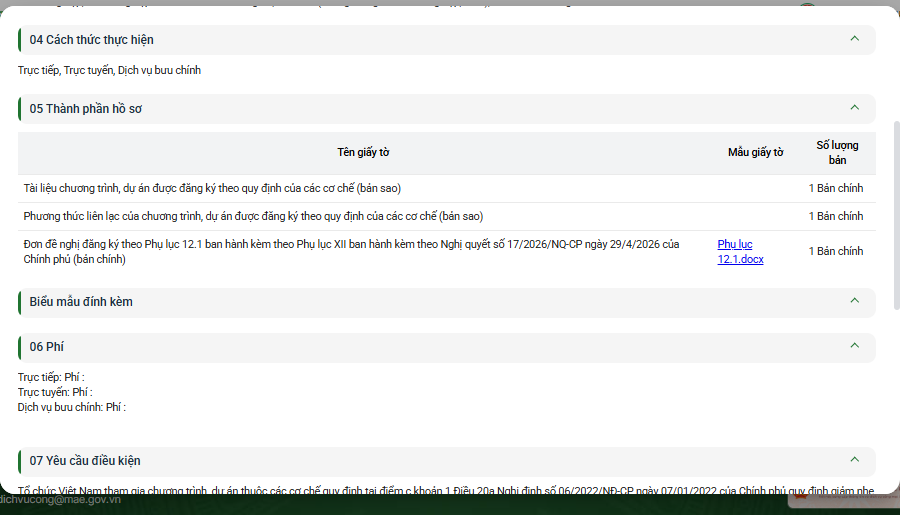
\includegraphics[width=0.68\textwidth]{image/dvc_1014129_ho_so.png}
        \caption{Thành phần hồ sơ}
    \end{subfigure}

    \vspace{0.3cm}
    \begin{subfigure}{\textwidth}
        \centering
        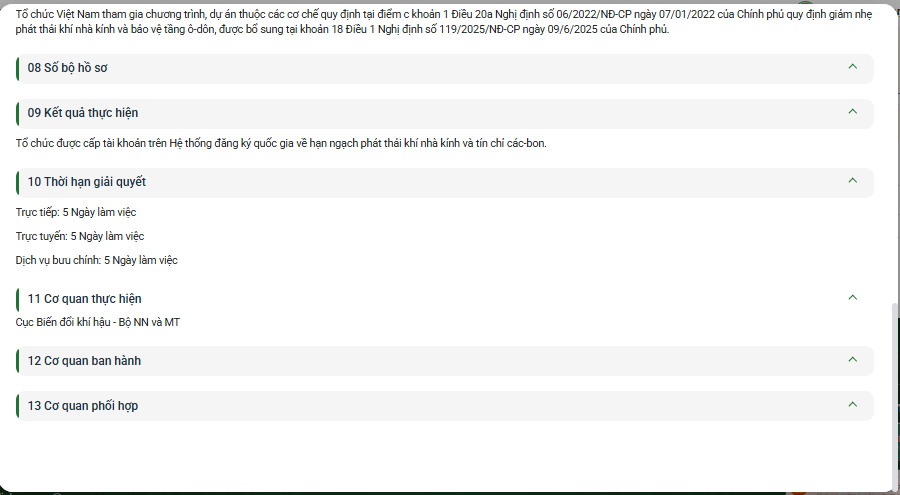
\includegraphics[width=0.68\textwidth]{image/dvc_1014129_thoi_han.png}
        \caption{Kết quả, thời hạn giải quyết và cơ quan thực hiện}
    \end{subfigure}
    \caption[Trang thủ tục đăng ký tài khoản trên Hệ thống đăng ký quốc gia]%
    {Trang thủ tục mã 1.014129 về đăng ký tài khoản trên Hệ thống đăng ký quốc gia, trên Hệ thống thông tin giải quyết thủ tục hành chính ngành Nông nghiệp và Môi trường (ảnh chụp màn hình, truy cập ngày 04/11/2026)~\cite{mae2026tthc1014129}.}
    \label{fig:ks-dvc-taikhoan}
\end{figure}

\begin{figure}[htbp]
    \centering
    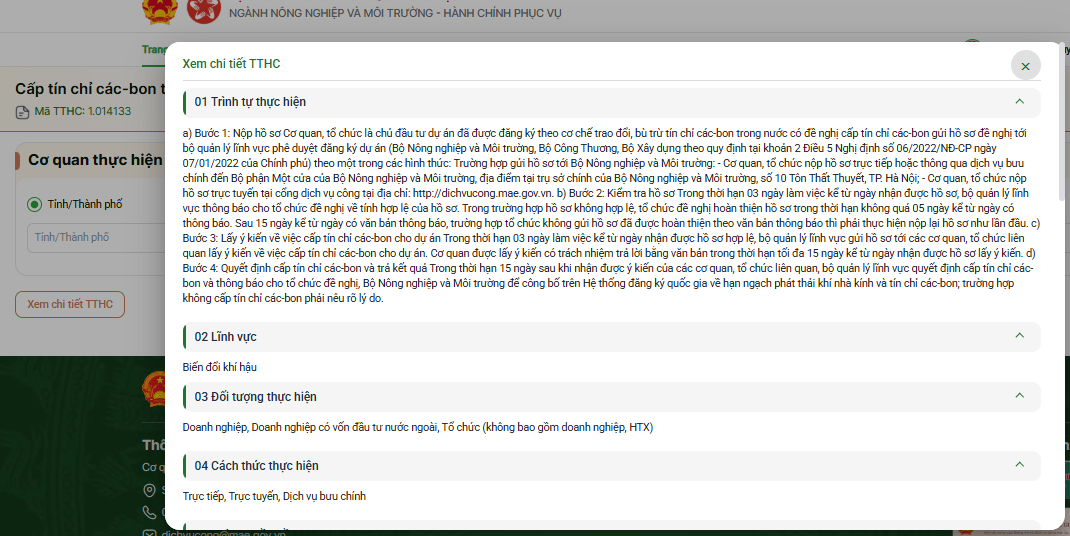
\includegraphics[width=0.9\textwidth]{image/dvc_1014133_trinh_tu.png}
    \caption[Trang thủ tục cấp tín chỉ các-bon]%
    {Trang thủ tục mã 1.014133 về cấp tín chỉ các-bon theo cơ chế trong nước: trình tự bốn bước theo quy định trước Nghị định 396/2026/NĐ-CP, từ nộp hồ sơ, kiểm tra, lấy ý kiến đến quyết định cấp (ảnh chụp màn hình, truy cập ngày 04/11/2026)~\cite{mae2026tthc1014133}.}
    \label{fig:ks-dvc-tinchi}
\end{figure}

\begin{figure}[htbp]
    \centering
    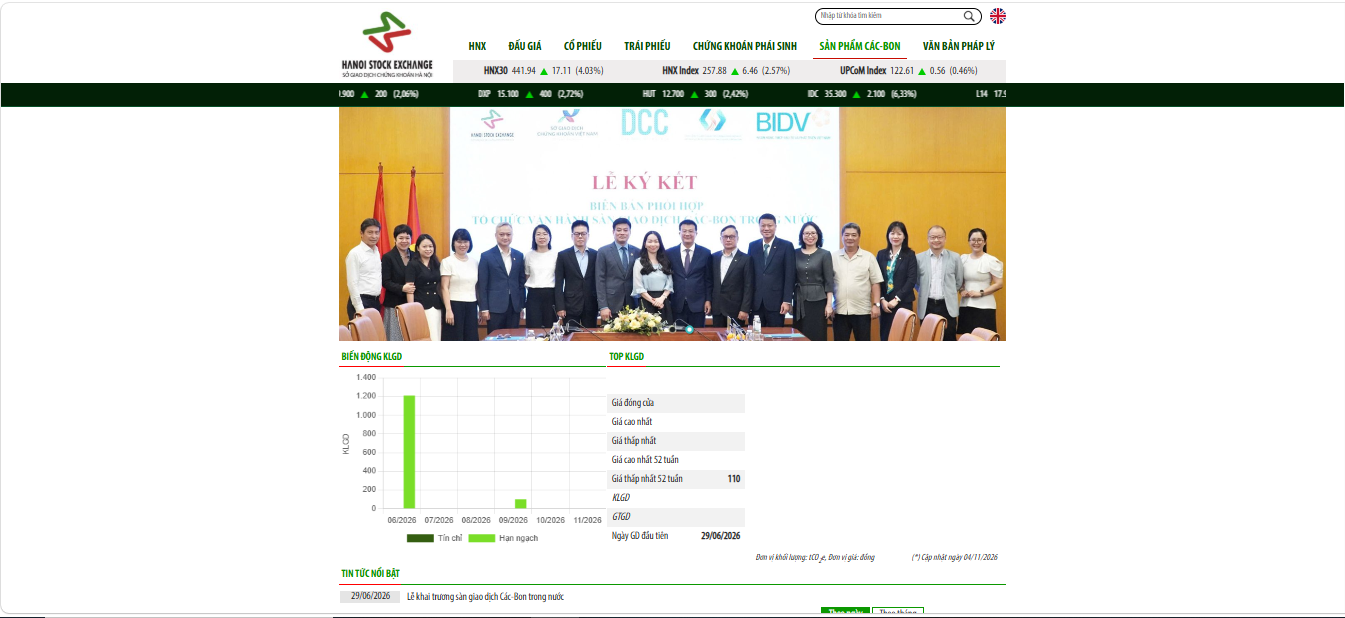
\includegraphics[width=\textwidth]{image/hnx_san_cacbon.png}
    \caption[Trang sản phẩm các-bon trên website của HNX]%
    {Trang sản phẩm các-bon trên website của HNX: biểu đồ khối lượng giao dịch theo tháng và thông tin mã VN2025 (ảnh chụp màn hình, truy cập ngày 04/11/2026)~\cite{hnx2026sanphamcacbon}.}
    \label{fig:ks-hnx}
\end{figure}

\begin{figure}[htbp]
    \centering
    \begin{subfigure}{\textwidth}
        \centering
        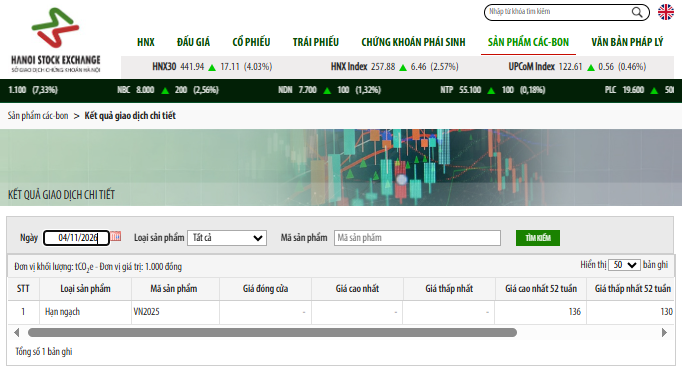
\includegraphics[width=0.75\textwidth]{image/hnx_ket_qua_giao_dich.png}
        \caption{Kết quả giao dịch chi tiết ngày 04/11/2026~\cite{hnx2026ketquagd}}
    \end{subfigure}

    \vspace{0.3cm}
    \begin{subfigure}{\textwidth}
        \centering
        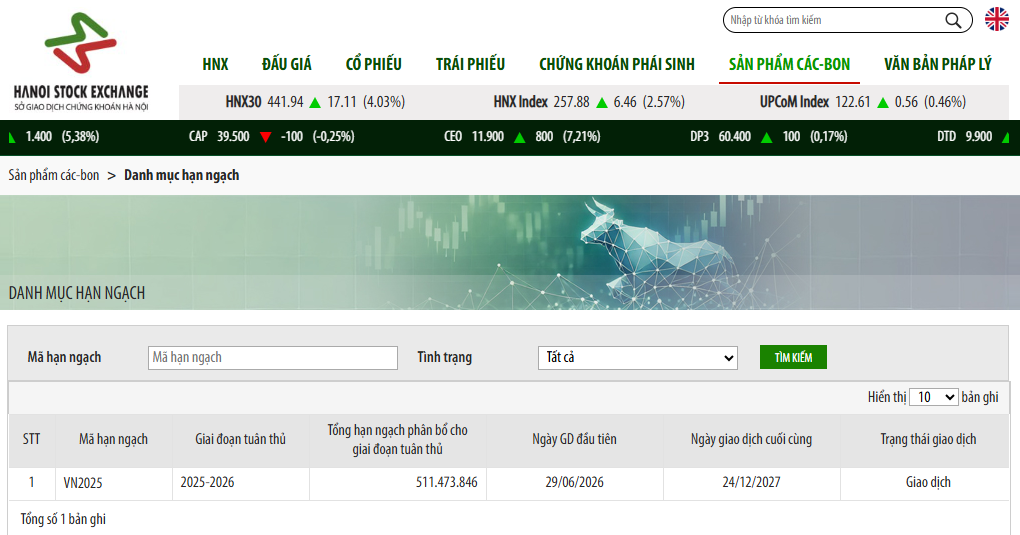
\includegraphics[width=0.85\textwidth]{image/hnx_danh_muc_han_ngach.png}
        \caption{Danh mục hạn ngạch~\cite{hnx2026danhmuchanngach}}
    \end{subfigure}
    \caption[Kết quả giao dịch và danh mục hạn ngạch trên website của HNX]%
    {Kết quả giao dịch và danh mục hạn ngạch trên trang sản phẩm các-bon của HNX (ảnh chụp màn hình, truy cập ngày 04/11/2026).}
    \label{fig:ks-hnx-chitiet}
\end{figure}

\begin{figure}[htbp]
    \centering
    \begin{subfigure}{\textwidth}
        \centering
        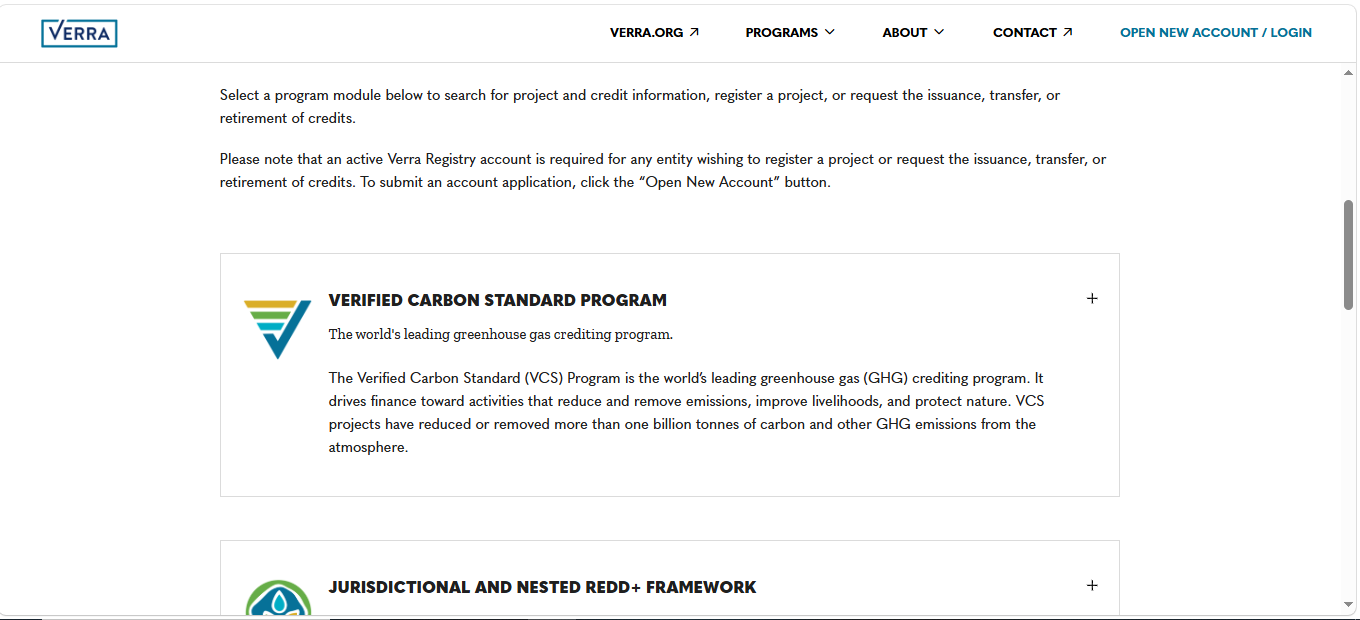
\includegraphics[width=0.9\textwidth]{image/verra_registry_home.png}
        \caption{Trang chủ: người dùng chọn chương trình để tra cứu, còn các nghiệp vụ đăng ký, phát hành, chuyển nhượng và hủy tín chỉ yêu cầu tài khoản~\cite{verraregistryhome}}
    \end{subfigure}

    \vspace{0.3cm}
    \begin{subfigure}{\textwidth}
        \centering
        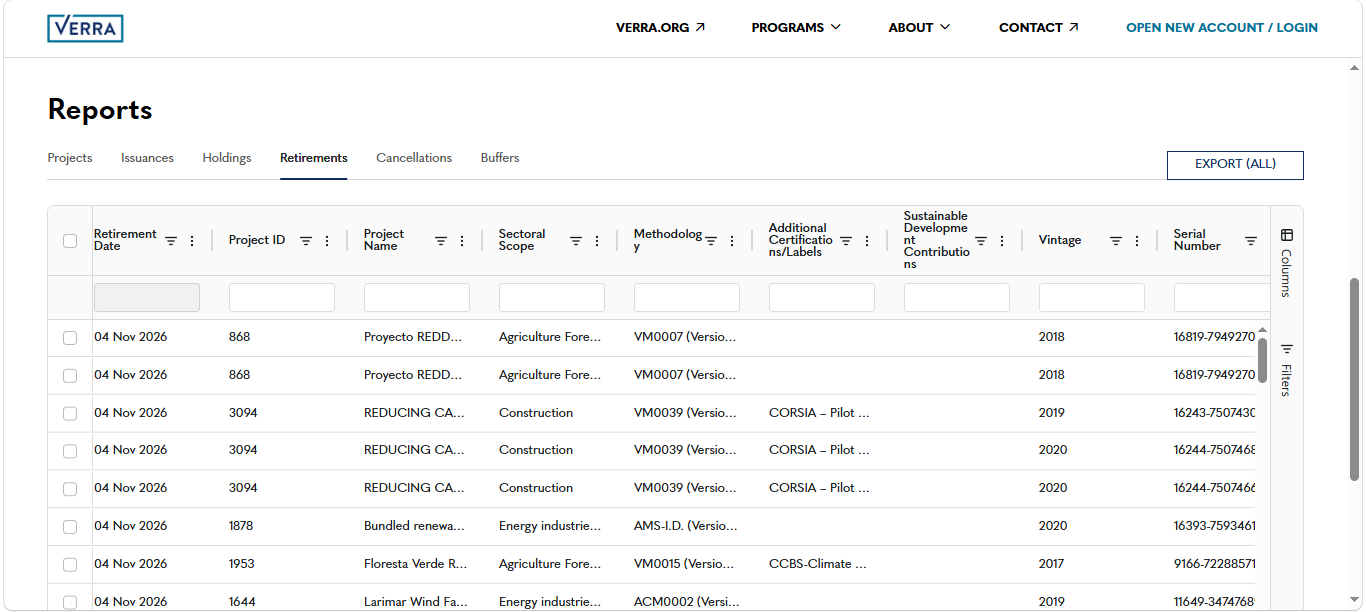
\includegraphics[width=0.9\textwidth]{image/verra_retirements.png}
        \caption{Báo cáo Retirements: mỗi dòng là một lô tín chỉ đã hủy, có ngày hủy, dự án, vintage và số sê-ri~\cite{verra2026retirements}}
    \end{subfigure}
    \caption[Trang công khai của Verra Registry]%
    {Trang công khai của Verra Registry (ảnh chụp màn hình, truy cập ngày 04/11/2026).}
    \label{fig:ks-verra}
\end{figure}

% [VIẾT SAU - ẢNH CHỤP] Thay bằng ảnh dashboard của Việt Nam (Southeast Asia -> Viet Nam) và sửa chú thích.
\begin{figure}[htbp]
    \centering
    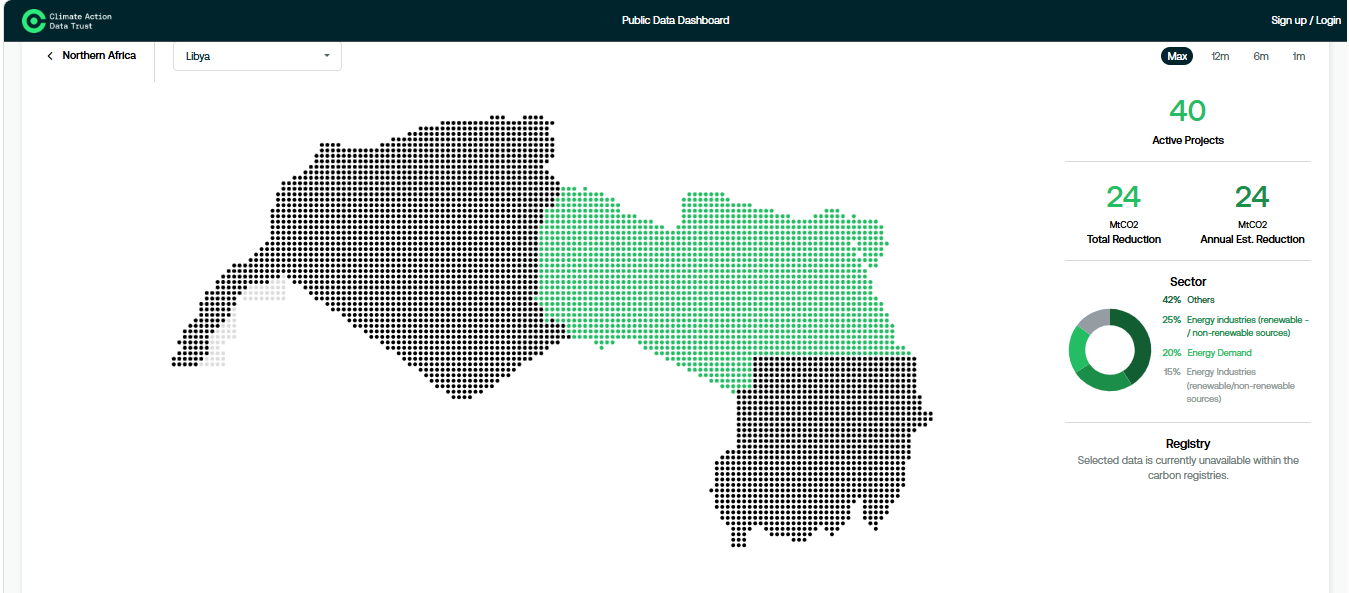
\includegraphics[width=0.9\textwidth]{image/cadtrust_dashboard.png}
    \caption[Public Data Dashboard của CAD Trust]%
    {Public Data Dashboard của CAD Trust: số liệu tổng hợp của Libya gồm số dự án, lượng giảm phát thải và cơ cấu theo lĩnh vực (ảnh chụp màn hình, truy cập ngày 04/11/2026)~\cite{cadtrust2026dashboard}.}
    \label{fig:ks-cadtrust}
\end{figure}

\begin{figure}[htbp]
    \centering
    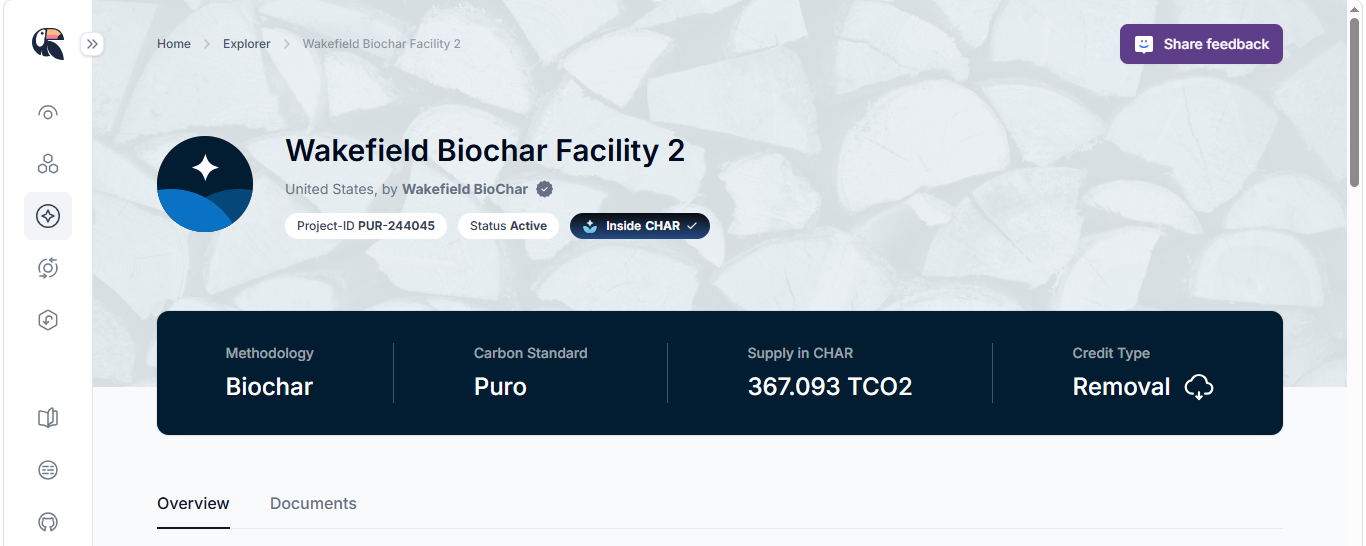
\includegraphics[width=0.9\textwidth]{image/toucan_project.png}
    \caption[Trang một dự án trên ứng dụng Toucan]%
    {Trang dự án Wakefield Biochar Facility 2 trên ứng dụng Toucan: mã dự án, tiêu chuẩn gốc, phương pháp luận, loại tín chỉ và pool chứa token (ảnh chụp màn hình, truy cập ngày 04/11/2026)~\cite{toucan2026wakefield}.}
    \label{fig:ks-toucan}
\end{figure}

Từ kết quả quan sát, có thể rút ra bốn nhận xét.

Thứ nhất, các nghiệp vụ trong nước được xử lý qua nhiều cấp phê duyệt và nhiều hệ thống: một giao dịch cần dữ liệu ở Hệ thống đăng ký quốc gia, hệ thống giao dịch của HNX, hệ thống lưu ký của VSDC và tài khoản tại công ty chứng khoán. Mỗi bước của thủ tục cấp tín chỉ có thời hạn riêng và có nhánh quay lại khi hồ sơ phải bổ sung hoặc nộp lại. Theo Nghị định 396/2026/NĐ-CP, từ ngày 12/12/2026 việc cấp tín chỉ theo cơ chế trong nước mất tối đa 26 ngày làm việc; quy trình cũ (06 ngày làm việc và 30 ngày) quy đổi ra khoảng 27 đến 28 ngày làm việc, nên thời hạn được rút ngắn khoảng một đến hai ngày làm việc. Thay đổi lớn hơn là thẩm quyền cấp tài khoản và cấp tín chỉ được phân cấp xuống cấp tỉnh: tín chỉ trong nước sẽ được cấp ở nhiều địa phương nhưng vẫn phải ghi nhận thống nhất trên Hệ thống đăng ký quốc gia. Đây là căn cứ để hệ thống mới cho phép nhiều tài khoản cùng có quyền phát hành, mỗi đơn vị cấp tỉnh một tài khoản (NC-09).

Thứ hai, thị trường chưa có thanh khoản: đến ngày 04/11/2026 chỉ có 7 giao dịch và hàng hóa duy nhất là hạn ngạch, nên chưa có dữ liệu thực tế về giao dịch tín chỉ trong nước để hệ thống của đồ án sử dụng.

Thứ ba, Verra Registry tách rõ phần tra cứu công khai và phần nghiệp vụ cần tài khoản; báo cáo hủy tín chỉ được công khai tới từng lô và số sê-ri, nhưng thông tin người thụ hưởng có thể được ẩn, cho thấy yêu cầu minh bạch luôn đi kèm giới hạn về riêng tư.

Thứ tư, các hệ thống quốc tế tổng hợp dữ liệu hoặc token hóa tín chỉ đều dựa vào hệ thống đăng ký gốc: CAD Trust chỉ hiển thị được số liệu mà các hệ thống đăng ký cung cấp, còn dự án được quan sát trên Toucan là tín chỉ do Puro cấp và vẫn giữ mã dự án của Puro. Vì vậy, mỗi bản ghi tín chỉ trên blockchain cần giữ liên kết tới mã dự án và số sê-ri do hệ thống đăng ký gốc cấp.

% [VIẾT SAU - PHỎNG VẤN CHUYÊN GIA] Phỏng vấn ngắn 1–2 chuyên gia (giảng viên/nhân viên đơn vị tư vấn các-bon,
% công ty chứng khoán là thành viên giao dịch các-bon). Mỗi buổi 20–30 phút, ghi chép, xin phép trước khi trích.
% Câu hỏi gợi ý, gắn với vấn đề:
%   Q1 (VĐ-1) Khi nhận một dự án đã đăng ký Verra/Gold Standard, đơn vị kiểm tra trùng đăng ký thế nào?
%   Q2 (VĐ-2) Doanh nghiệp đang chứng minh với đối tác nước ngoài rằng tín chỉ đã hủy bằng giấy tờ gì?
%   Q3 (VĐ-3) Báo cáo thẩm định được lưu, chia sẻ, ký như thế nào; đã gặp trường hợp hồ sơ bị sửa sau khi cấp chưa?
%   Q4 (VĐ-4) Việc đối soát giữa Hệ thống đăng ký quốc gia, HNX, VSDC tốn bao nhiêu nhân lực/thời gian; sai lệch thường gặp?
%   Q5 (VĐ-5) Vì sao thanh khoản thấp; khi nào tín chỉ trong nước dự kiến được đưa lên sàn?
%   Q6 (chung) Nếu có một công cụ cho phép bên thứ ba tự tra cứu lịch sử tín chỉ, dữ liệu nào được phép công khai?
% Kết quả: thêm cột "Ý kiến chuyên gia" vào Bảng tab:ks-doituong và cập nhật mục Những khó khăn và tồn tại.

% ------------------------------------------------------------
\FloatBarrier
\subsection*{Đánh giá hệ thống hiện tại}
\label{subsec:ks-danhgia}

\subsubsection*{Ưu điểm}

Hệ thống đăng ký quốc gia và hạ tầng sàn giao dịch có nhiều ưu điểm về mặt quản lý:
\begin{itemize}
    \item Có cơ sở pháp lý rõ ràng và dữ liệu gốc thống nhất: Bộ Nông nghiệp và Môi trường là cơ quan duy nhất cấp mã và số sê-ri; dữ liệu trên hệ thống đăng ký là dữ liệu gốc để đối chiếu khi có sai lệch~\cite{vietnam2026thongtu11}. Điều này hạn chế việc cùng một lượng giảm phát thải được ghi nhận nhiều lần trong phạm vi trong nước.
    \item Định danh tới từng đơn vị: mỗi tấn CO$_2$e có số sê-ri riêng; mã trong nước không được cấp lại sau khi hủy~\cite{vietnam2026thongtu11}.
    \item Mô hình trạng thái chặt chẽ: tám tiểu khoản phản ánh đầy đủ các trạng thái trong vòng đời, kể cả các trường hợp đặc thù như vay mượn, chuyển giao giữa các giai đoạn và phong tỏa.
    \item Định danh pháp lý và kiểm soát nội bộ: tài khoản gắn với mã số thuế, xác thực qua Cổng dịch vụ công quốc gia và có cơ chế tạo, duyệt giao dịch, nên trách nhiệm pháp lý của từng giao dịch được xác định rõ.
    \item Tích hợp với hạ tầng tài chính sẵn có: sàn giao dịch tận dụng kinh nghiệm vận hành thị trường chứng khoán của HNX và VSDC; giai đoạn thí điểm được miễn phí dịch vụ~\cite{vietnam2026nghidinh29}.
\end{itemize}
Các hệ thống quốc tế cũng có những ưu điểm mà đồ án tham khảo: Verra có quy trình đã vận hành lâu năm và trang tra cứu công khai~\cite{verra2024vcs}; UNDP National Carbon Registry là mã nguồn mở và hỗ trợ báo cáo theo Điều~6~\cite{undp2024nationalregistry}; CAD Trust tạo mô hình dữ liệu chung giữa nhiều hệ thống đăng ký~\cite{cadtrust2025datamodel}; Toucan cho thấy việc hủy tín chỉ có thể được ghi công khai trên blockchain và kiểm chứng bởi bất kỳ ai~\cite{toucan2025docs}.

\subsubsection*{Nhược điểm}

Bảng~\ref{tab:ks-uunhuoc} tóm tắt ưu điểm và nhược điểm của từng hệ thống được khảo sát.
% [VIẾT SAU] Khi viết xong mục Đánh giá và khoảng trống (Chương 2), thêm lại:
% So sánh chi tiết theo các tiêu chí kỹ thuật được trình bày ở mục \ref{subsec:khoangtrong}.

\begin{table}[htbp]
    \centering
    \caption{Ưu điểm và nhược điểm của các hệ thống được khảo sát}
    \label{tab:ks-uunhuoc}
    \small
    \renewcommand{\arraystretch}{1.2}
    \begin{tabularx}{\textwidth}{|p{2.6cm}|X|X|}
        \hline
        \textbf{Hệ thống} & \textbf{Ưu điểm} & \textbf{Nhược điểm} \\
        \hline
        Hệ thống đăng ký quốc gia và sàn giao dịch trong nước & Pháp lý rõ ràng; dữ liệu gốc thống nhất; số sê-ri tới từng đơn vị; tám tiểu khoản; xác thực định danh điện tử~\cite{vietnam2026thongtu11} & Mới vận hành, đang thí điểm; ba hệ thống riêng phải đối soát cuối ngày; thông tin công khai chủ yếu ở dạng tổng hợp theo kỳ; bên ngoài không tự kiểm chứng được lịch sử của một tín chỉ \\
        \hline
        Verra Registry & Quy mô lớn nhất thị trường tự nguyện; số sê-ri duy nhất; tra cứu công khai; Project Hub số hóa hồ sơ~\cite{verra2024vcs} \cite{verra2024projecthub} & Tập trung, người dùng phải tin vào một đơn vị vận hành; chưa công bố API công khai~\cite{verraregistry}; không liên thông trực tiếp với hệ thống đăng ký khác \\
        \hline
        UNDP National Carbon Registry & Mã nguồn mở; hỗ trợ Điều~6 và báo cáo AEF; quản lý tách dãy sê-ri~\cite{undp2024nationalregistry} & Mỗi quốc gia phải tự triển khai, vận hành hạ tầng đám mây; sổ cái vẫn do một bên quản lý \\
        \hline
        CAD Trust & Liên thông nhiều hệ thống đăng ký; mô hình dữ liệu chung V2.0; mã băm trên blockchain Chia giúp phát hiện dữ liệu bị sửa~\cite{cadtrust2025datamodel} & Chỉ là lớp siêu dữ liệu, không ghi quyền sở hữu và không thực hiện giao dịch; mã băm chứng minh dữ liệu không bị sửa, không chứng minh dữ liệu đúng \\
        \hline
        Toucan Protocol & Token hóa tăng thanh khoản; hủy tín chỉ và chứng nhận hủy ghi công khai on-chain~\cite{toucan2025docs} & Phụ thuộc hệ thống đăng ký gốc; cầu nối từ Verra đã ngừng do Verra không chấp nhận token hóa tín chỉ đã hủy~\cite{toucan2025docs} \cite{spglobal2022verra}; pool token làm mất thông tin riêng của từng dự án \\
        \hline
    \end{tabularx}
\end{table}
\FloatBarrier

Đối với hệ thống trong nước, các nhược điểm chính được rút ra như sau:
\begin{itemize}
    \item Tính toàn vẹn dựa vào niềm tin vào đơn vị vận hành: các ràng buộc như ``mã trong nước không được cấp lại sau khi hủy'' hay ``không hủy quá số dư'' được bảo đảm bởi phần mềm và quy trình của cơ quan quản lý. Bên mua hoặc tổ chức bên ngoài không có công cụ để tự kiểm chứng rằng một số sê-ri chưa từng được cấp cho người khác hoặc chưa từng bị hủy.
    \item Dữ liệu phân tán giữa nhiều hệ thống: cùng một lượng tín chỉ được ghi nhận ở Hệ thống đăng ký quốc gia (tiểu khoản Số dư giao dịch) và ở hệ thống lưu ký của VSDC, nên phải đối soát định kỳ cuối mỗi ngày và có quy trình xử lý sai lệch~\cite{vietnam2026thongtu11}.
    \item Độ trễ trong nghiệp vụ: nhiều nghiệp vụ được xử lý theo ngày làm việc, chẳng hạn ký gửi chờ tổng hợp cuối ngày và chờ VSDC xác nhận trong 01 ngày làm việc; hủy tự nguyện được xử lý trong 02 ngày làm việc~\cite{vietnam2026thongtu11}.
    \item Mức độ công khai hạn chế: dữ liệu công bố chủ yếu là danh sách dự án và số liệu tổng hợp theo tháng, năm; thông tin giao dịch được bảo mật~\cite{vietnam2026thongtu11}. Điều này phù hợp yêu cầu bảo mật, nhưng khiến bên thứ ba khó truy vết lịch sử của một tín chỉ cụ thể. Định dạng dữ liệu trao đổi giữa các hệ thống được quy định trong tài liệu kỹ thuật nội bộ; tại thời điểm khảo sát, đồ án chưa tìm thấy tài liệu API công khai dành cho bên thứ ba.
    \item Khâu MRV chưa được số hóa đồng bộ: hồ sơ dự án, báo cáo giám sát và báo cáo thẩm định vẫn là các tệp tài liệu được nộp qua từng bước, chưa gắn với tín chỉ được cấp bằng một dấu vết kiểm chứng được.
\end{itemize}

\subsubsection*{Những khó khăn và tồn tại}

Từ các nhược điểm trên, đồ án xác định năm vấn đề (ký hiệu VĐ-1 đến VĐ-5) làm cơ sở cho nhu cầu xây dựng hệ thống mới được trình bày tiếp theo:
\begin{enumerate}[label=VĐ-\arabic*., leftmargin=1.6cm]
    \item Rủi ro tính toán kép giữa các hệ thống: hệ thống trong nước và các chương trình quốc tế (Verra, Gold Standard, các cơ chế Điều~6) sử dụng các không gian định danh khác nhau: mã trong nước song song với số sê-ri của từng chương trình. Nếu không có liên thông dữ liệu, cùng một dự án có thể được đăng ký ở nhiều nơi (phát hành kép)~\cite{schneider2019double}.
    \item Bên mua khó chứng minh tín chỉ đã được hủy: doanh nghiệp dùng tín chỉ để bù trừ phát thải hoặc để báo cáo với đối tác nước ngoài cần một bằng chứng có thể kiểm tra độc lập; hiện bằng chứng chủ yếu là thông báo xác nhận do cơ quan quản lý gửi cho chủ tài khoản.
    \item Hồ sơ MRV và thẩm định không gắn chặt với tín chỉ: không có cơ chế kỹ thuật bảo đảm rằng hồ sơ dùng để cấp tín chỉ không bị thay đổi sau khi cấp, hoặc không được dùng lại cho một lần cấp khác.
    \item Chi phí đối soát giữa nhiều cơ sở dữ liệu: cùng một lượng hạn ngạch, tín chỉ được ghi nhận đồng thời ở Hệ thống đăng ký quốc gia, hệ thống giao dịch của HNX và hệ thống lưu ký của VSDC, nên các bên phải gửi báo cáo, đối soát cuối mỗi ngày và duy trì quy trình xử lý sai lệch (Điều~23)~\cite{vietnam2026thongtu11}. Mỗi bên liên quan phải tin vào số liệu của bên kia hoặc tự đối chiếu lại. Thời gian xử lý tính theo ngày làm việc và qua nhiều cấp phê duyệt (phần quan sát ở trên) là hệ quả đi kèm, không phải vấn đề chính.
    \item Thị trường còn ở giai đoạn đầu: đến ngày 04/11/2026, sàn mới ghi nhận 7 giao dịch với 1.310 hạn ngạch, VN2025 là mã duy nhất được giao dịch và chưa có tín chỉ nào được đưa lên sàn~\cite{dantri2026san3thang} \cite{hnx2026sanphamcacbon}; giai đoạn thí điểm kéo dài đến hết năm 2028~\cite{vietnam2025qd232} \cite{dbnd2026santhuong}. Các quy định còn đang được sửa đổi, chẳng hạn Nghị định 396/2026/NĐ-CP phân cấp việc cấp tín chỉ theo cơ chế trong nước cho cấp tỉnh~\cite{vietnam2026nghidinh396}, nên hệ thống mới cần linh hoạt để thay đổi theo quy định.
\end{enumerate}
% [VIẾT SAU - PHỎNG VẤN] Câu cũ: "Cũng cần lưu ý rằng các tồn tại trên được rút ra từ tài liệu, chưa được
% kiểm chứng bằng phỏng vấn người dùng thực tế (mục \ref{subsubsec:ks-phuongphap})."
% -> sau khi phỏng vấn, bổ sung ý kiến của người dùng để xác nhận/điều chỉnh VĐ-1..VĐ-5.

% ------------------------------------------------------------
\FloatBarrier
\subsection*{Nhu cầu xây dựng hệ thống mới}
\label{subsec:ks-nhucau}

Hệ thống mới không nhằm thay thế Hệ thống đăng ký quốc gia, vốn là hệ thống có cơ sở pháp lý và giữ dữ liệu gốc. Đồ án định vị hệ thống của mình là một \emph{nguyên mẫu bổ sung}: thử nghiệm việc dùng smart contract để biến các ràng buộc nghiệp vụ đã được quy định (số sê-ri duy nhất, không hủy hai lần, không chuyển nhượng tín chỉ đã hủy) thành ràng buộc kỹ thuật mà bất kỳ ai cũng có thể kiểm chứng.

\subsubsection*{Nhu cầu chức năng}

Bảng~\ref{tab:ks-nhucauchucnang} liệt kê các nhu cầu chức năng, kèm vấn đề mà mỗi nhu cầu giải quyết. Ghi chú ``một phần'' nghĩa là nhu cầu chỉ giải quyết vấn đề trong phạm vi của chính hệ thống (ví dụ không phát hành trùng dãy sê-ri trong hệ thống), chưa ngăn được việc một dự án đăng ký ở hệ thống khác. Dấu ``--'' nghĩa là nhu cầu phục vụ vận hành của hệ thống, không trực tiếp giải quyết vấn đề nào.
% [VIẾT SAU] Khi viết xong mục Yêu cầu chức năng (Chương 3), thêm lại:
% Các nhu cầu này được chi tiết hóa thành yêu cầu chức năng ở mục \ref{subsec:ycchucnang}.

\begin{table}[htbp]
    \centering
    \caption{Nhu cầu chức năng của hệ thống mới}
    \label{tab:ks-nhucauchucnang}
    \small
    \renewcommand{\arraystretch}{1.2}
    \begin{tabularx}{\textwidth}{|p{1.3cm}|X|>{\raggedright\arraybackslash}p{2.8cm}|>{\raggedright\arraybackslash}p{2.1cm}|}
        \hline
        \textbf{Mã} & \textbf{Nhu cầu} & \textbf{Bên liên quan} & \textbf{Vấn đề} \\
        \hline
        NC-01 & Đăng ký dự án và tải lên hồ sơ (PDD, báo cáo giám sát), lưu mã băm của hồ sơ & Chủ dự án & VĐ-3 \\
        \hline
        NC-02 & Gửi yêu cầu cấp tín chỉ; VVB xem hồ sơ, phê duyệt hoặc từ chối & Chủ dự án, VVB & VĐ-3 \\
        \hline
        NC-03 & Phát hành lô tín chỉ có dãy số sê-ri duy nhất; từ chối phát hành trùng dãy sê-ri hoặc dùng lại hồ sơ đã dùng & Cơ quan quản lý (sau khi VVB phê duyệt) & VĐ-1 (một phần), VĐ-3 \\
        \hline
        NC-04 & Chuyển nhượng tín chỉ giữa các ví, ghi lịch sử sở hữu công khai & Chủ dự án, doanh nghiệp & VĐ-2, VĐ-4 \\
        \hline
        NC-05 & Giao dịch từng phần của một lô thông qua token có thể thay thế (pool) & Chủ dự án, doanh nghiệp & -- \\
        \hline
        NC-06 & Hủy tín chỉ trực tiếp từ lô hoặc từ pool, ghi người thụ hưởng và dãy sê-ri cụ thể bị hủy trong cả hai trường hợp; tín chỉ đã hủy không chuyển nhượng hoặc hủy lại được & Doanh nghiệp & VĐ-2 \\
        \hline
        NC-07 & Tra cứu công khai tín chỉ theo số sê-ri và xem chứng nhận hủy, có liên kết tới giao dịch on-chain & Người dùng công khai & VĐ-2 \\
        \hline
        NC-08 & Dashboard so sánh lượng tín chỉ đã hủy với lượng phát thải hoặc hạn ngạch đã khai báo & Doanh nghiệp & VĐ-2 \\
        \hline
        NC-09 & Quản lý vai trò: cấp, thu hồi quyền VVB và quyền phát hành; cho phép nhiều tài khoản cùng có quyền phát hành (mỗi đơn vị cấp tỉnh một tài khoản, theo Nghị định 396/2026/NĐ-CP) và ghi lại tài khoản đã phát hành từng lô; tạm dừng hệ thống khi có sự cố & Cơ quan quản lý (cấp bộ, cấp tỉnh) & VĐ-5 \\
        \hline
        NC-10 & Xuất dữ liệu dự án, đợt cấp, đơn vị tín chỉ theo cấu trúc CAD Trust V2.0 & Cơ quan quản lý, hệ thống bên ngoài & VĐ-1 (một phần) \\
        \hline
    \end{tabularx}
\end{table}

\subsubsection*{Nhu cầu phi chức năng}

\begin{itemize}
    \item Toàn vẹn dữ liệu: mỗi dãy số sê-ri chỉ được phát hành một lần; quyền sở hữu và trạng thái hủy lấy dữ liệu on-chain làm gốc; dữ liệu off-chain có thể dựng lại từ các sự kiện on-chain.
    \item Minh bạch và kiểm chứng được: bên thứ ba có thể tự kiểm tra lịch sử của một tín chỉ (dãy sê-ri, trạng thái, các lần chuyển nhượng và hủy) mà không cần xin dữ liệu từ đơn vị vận hành; phạm vi dữ liệu được công khai giới hạn theo nhu cầu riêng tư dưới đây.
    \item Bảo mật và phân quyền: chỉ tài khoản có vai trò phù hợp mới được phát hành tín chỉ hoặc thay đổi vai trò; khóa riêng của người dùng không rời khỏi ví; smart contract được bảo vệ trước các lỗ hổng phổ biến như reentrancy.
    \item Riêng tư: Thông tư 11/2026/TT-BNNMT vừa yêu cầu bảo đảm tính công khai, minh bạch (Điều~4), vừa yêu cầu các tổ chức tham gia bảo mật thông tin truy cập, thông tin giao dịch (Điều~24)~\cite{vietnam2026thongtu11}. Hai yêu cầu này được dung hòa bằng cách chỉ công khai phần dữ liệu cần để kiểm chứng: on-chain chỉ ghi địa chỉ ví (không gắn trực tiếp với tên hay mã số thuế của doanh nghiệp), dãy sê-ri, trạng thái và mã băm hồ sơ; thông tin định danh doanh nghiệp, hồ sơ dự án và giá giao dịch lưu off-chain có phân quyền. Cách làm này tương tự CAD Trust, vốn chỉ đưa mã băm lên blockchain~\cite{cadtrust2025datamodel}, và Verra Registry, nơi số sê-ri của tín chỉ đã hủy được công khai nhưng chủ tài khoản có thể ẩn người thụ hưởng và lý do hủy~\cite{verra2020registryv2}. Khi áp dụng thực tế, có thể thay mạng công khai bằng blockchain có cấp phép (permissioned) do các cơ quan liên quan cùng vận hành; đồ án dùng testnet công khai vì đây là nguyên mẫu với dữ liệu mô phỏng.
    \item Chi phí: chi phí gas cho các thao tác phát hành, chuyển nhượng và hủy phải được đo và ở mức chấp nhận được.
    \item Tương thích dữ liệu: cấu trúc dữ liệu off-chain bám theo mô hình CAD Trust V2.0 để có thể trao đổi với hệ thống khác.
    \item Dễ sử dụng và dễ mở rộng: giao diện web cho từng vai trò; kiến trúc tách lớp để có thể bổ sung sau này các chức năng như ký số của VVB, kết nối dữ liệu MRV tự động, hay ánh xạ sang mã trong nước của Thông tư 11/2026/TT-BNNMT.
\end{itemize}

\subsubsection*{Định hướng giải pháp}

Từ các nhu cầu trên, đồ án lựa chọn giải pháp theo kiến trúc lai on-chain và off-chain:
% [VIẾT SAU] Khi khôi phục Chương 3: thêm ", được trình bày chi tiết ở mục \ref{sec:kientruc}" trước dấu hai chấm.
\begin{itemize}
    \item Ba thao tác cần kiểm chứng công khai (phát hành, chuyển nhượng, hủy) được thực hiện bằng smart contract trên Ethereum: mỗi lô tín chỉ là một NFT ERC-721 lưu dãy sê-ri và mã băm hồ sơ; pool ERC-20 cho giao dịch từng phần; hàm hủy đốt token và ghi người thụ hưởng.
    \item Hồ sơ, thông tin dự án và tài khoản người dùng được lưu trong cơ sở dữ liệu quan hệ theo mô hình CAD Trust V2.0; một tiến trình đồng bộ đọc sự kiện từ smart contract để cập nhật cơ sở dữ liệu.
    \item Hệ thống được xây dựng ở mức nguyên mẫu, triển khai trên testnet Sepolia, dùng dữ liệu mô phỏng và không kết nối với Hệ thống đăng ký quốc gia hay Verra Registry.
\end{itemize}
Các ý tưởng từ hệ thống trong nước được giữ lại trong thiết kế: định danh theo lô với dãy số sê-ri (giống mã trong nước và số sê-ri), phân tách người tạo yêu cầu và người phê duyệt (giống cơ chế tạo và duyệt giao dịch), VVB chỉ phê duyệt kết quả thẩm định còn cơ quan quản lý mới phát hành tín chỉ (giống quy trình cơ quan có thẩm quyền quyết định cấp tín chỉ sau khi có báo cáo thẩm định~\cite{mae2025qd2935} \cite{vietnam2026nghidinh396}), và khả năng tạm dừng hệ thống khi có sự cố (giống quy định quản lý sự cố của Thông tư 11/2026/TT-BNNMT).

% ------------------------------------------------------------
\FloatBarrier
\subsection*{Kết luận và đánh giá tính khả thi sơ bộ}
\label{subsec:ks-khathi}

Kết quả khảo sát cho thấy Việt Nam đã có hạ tầng pháp lý và kỹ thuật tương đối đầy đủ cho thị trường các-bon trong nước: Hệ thống đăng ký quốc gia giữ dữ liệu gốc và sàn giao dịch đã đi vào hoạt động. Khoảng trống mà đồ án hướng tới không phải là việc thiếu một hệ thống quản lý, mà là việc các ràng buộc chống tính toán kép đang được bảo đảm bằng niềm tin vào đơn vị vận hành và bằng đối soát giữa nhiều cơ sở dữ liệu, trong khi bên ngoài khó tự kiểm chứng. Bảng~\ref{tab:ks-khathi} đánh giá sơ bộ tính khả thi của việc xây dựng hệ thống trong phạm vi một đồ án tốt nghiệp.

\begin{table}[htbp]
    \centering
    \caption{Đánh giá tính khả thi sơ bộ}
    \label{tab:ks-khathi}
    \small
    \renewcommand{\arraystretch}{1.2}
    \begin{tabularx}{\textwidth}{|p{2.4cm}|X|X|}
        \hline
        \textbf{Khía cạnh} & \textbf{Đánh giá} & \textbf{Rủi ro và cách xử lý} \\
        \hline
        Kỹ thuật & Các công nghệ cần dùng (Solidity, OpenZeppelin, Hardhat, Node.js, PostgreSQL, Next.js) đều là mã nguồn mở, có tài liệu đầy đủ; chuẩn ERC-721, ERC-20 đã ổn định & Lỗi smart contract không sửa được sau khi triển khai: dùng thư viện đã được kiểm toán, viết kiểm thử đơn vị, quét bằng công cụ phân tích tĩnh \\
        \hline
        Kinh tế & Testnet Sepolia và các công cụ phát triển không mất phí; không cần mua phần cứng & Chi phí gas trên mạng chính chưa xác định: đo gas từng thao tác khi kiểm thử \\
        % [VIẾT SAU] Khi có Chương 5: "đo gas từng thao tác ở Chương~\ref{chap:ketqua}"
        \hline
        Vận hành & Người dùng thao tác qua giao diện web và ví MetaMask & Người dùng chưa quen với ví điện tử: giao diện hướng dẫn từng bước, các vai trò được phân tách rõ \\
        \hline
        Pháp lý & Hệ thống là nguyên mẫu nghiên cứu, không phát hành tín chỉ thật, không thay thế Hệ thống đăng ký quốc gia & Token trên testnet không có giá trị; việc áp dụng thực tế cần cơ chế pháp lý riêng, ghi vào hướng phát triển \\
        \hline
        Thời gian & Phạm vi bám theo phiếu giao nhiệm vụ; lộ trình 9 tuần có mốc kiểm tra & Trễ tiến độ: có các mốc cắt phạm vi (bỏ pool hoặc dashboard nếu cần) \\
        \hline
    \end{tabularx}
\end{table}

Từ kết quả đánh giá, việc xây dựng hệ thống ở mức nguyên mẫu là khả thi trong thời gian thực hiện đồ án. Kết quả khảo sát sơ bộ được dùng làm đầu vào cho phần phát biểu bài toán và mục tiêu ở mục \ref{sec:nhiemvu} và cho phần phân tích yêu cầu ở các chương sau.
% [VIẾT SAU] Khi khôi phục Chương 3: "ở Chương~\ref{chap:thietke}" thay cho "ở các chương sau".
% [VIẾT SAU - PHỎNG VẤN] Câu cũ: "Khi có điều kiện, các nhận định ở mục \ref{subsec:ks-danhgia} cần được
% kiểm chứng thêm bằng phỏng vấn các đối tượng trong Bảng~\ref{tab:ks-doituong}."

% ------------------------------------------------------------
\section{Nhiệm vụ đồ án}
\label{sec:nhiemvu}
% Khoa yêu cầu mục này nêu: tính cấp thiết, lý do chọn đề tài, ý nghĩa khoa học và thực tiễn,
% mục tiêu, đối tượng, phạm vi giới hạn. Bám sát phiếu giao nhiệm vụ (mục A1, B1–B3).

\subsection*{Phát biểu bài toán}
\label{subsec:baitoan}
% Từ khảo sát ở các mục \ref{sec:dongluc}–\ref{sec:vietnam}, rút ra 3–4 vấn đề cụ thể mà hệ thống
% phải giải quyết, mỗi vấn đề trỏ về đúng mục đã khảo sát. Gợi ý:
%  - double counting (bán kép, phát hành kép, tuyên bố kép);
%  - khó kiểm chứng nguồn gốc và lịch sử sở hữu của một tín chỉ;
%  - dữ liệu phân mảnh giữa các hệ thống đăng ký, chưa theo mô hình chung (CAD Trust);
%  - việc hủy tín chỉ (retire) khó kiểm chứng công khai.
Từ các nội dung khảo sát ở các mục \ref{sec:dongluc}--\ref{sec:khaosatsobo}, đồ án xác định bốn vấn đề mà một hệ thống quản lý tín chỉ các-bon cần giải quyết:
\begin{enumerate}
    \item Tính toán kép: cùng một lượng giảm phát thải có thể bị cấp tín chỉ nhiều lần (phát hành kép), cùng một tín chỉ có thể bị bán hoặc sử dụng nhiều lần (sử dụng kép), hoặc được nhiều bên cùng tuyên bố (tuyên bố kép)~\cite{schneider2019double}. Các dạng này đã được trình bày ở mục \ref{sec:dongluc}.
    \item Khó kiểm chứng nguồn gốc và lịch sử sở hữu: ở các hệ thống đăng ký tập trung như Verra Registry hay Hệ thống đăng ký quốc gia, dữ liệu sở hữu do một đơn vị quản lý; bên ngoài chỉ tra cứu được những gì đơn vị đó công bố và không tự kiểm chứng được lịch sử của một tín chỉ (mục \ref{sec:sodangky} và mục \ref{sec:khaosatsobo}).
    \item Dữ liệu phân mảnh: mỗi hệ thống đăng ký dùng định dạng và không gian định danh riêng; mô hình dữ liệu chung như CAD Trust V2.0 mới được công bố và đang được các thành viên áp dụng (mục \ref{sec:sodangky}).
    \item Việc hủy tín chỉ khó kiểm chứng công khai: bằng chứng hủy chủ yếu là xác nhận của đơn vị vận hành hệ thống đăng ký; bên mua khó đưa ra một bằng chứng mà bên thứ ba có thể tự kiểm tra (mục \ref{sec:khaosatsobo}).
\end{enumerate}
Bài toán của đồ án là xây dựng một hệ thống quản lý tín chỉ các-bon, trong đó các thao tác phát hành, chuyển nhượng và hủy tín chỉ được thực hiện bằng smart contract trên blockchain Ethereum, sao cho mỗi dãy số sê-ri chỉ được phát hành một lần, tín chỉ đã hủy không thể bị chuyển nhượng hay hủy lại, và bất kỳ ai cũng có thể kiểm chứng lịch sử của một tín chỉ. Dữ liệu dự án và hồ sơ được lưu off-chain theo mô hình dữ liệu CAD Trust V2.0.

\subsection*{Mục tiêu của đồ án}
\label{subsec:muctieu}
% Lấy từ phiếu (B1–B3), viết thành các mục tiêu kiểm tra được để Chương 5 đối chiếu lại:
%  - smart contract: Minting (ERC-721), Trading (pool ERC-20), Retirement (burn, chống double counting);
%  - CSDL off-chain theo CAD Trust V2.0; API RESTful; giao diện Next.js + MetaMask; dashboard.
Mục tiêu tổng quát của đồ án là xây dựng một nguyên mẫu hệ thống quản lý vòng đời tín chỉ các-bon (phát hành, giao dịch, hủy) trên blockchain Ethereum, có khả năng ngăn tính toán kép trong phạm vi hệ thống. Các mục tiêu cụ thể gồm:
\begin{enumerate}
    \item Smart contract:
    \begin{itemize}
        \item Phát hành (Minting): mỗi lô tín chỉ là một NFT ERC-721 lưu dự án, năm vintage, dãy số sê-ri, số lượng và mã băm hồ sơ; VVB thẩm định và phê duyệt hồ sơ, sau đó cơ quan quản lý (vai trò phát hành) mới được phát hành lô tín chỉ; smart contract từ chối dãy sê-ri trùng và hồ sơ đã được dùng.
        \item Giao dịch (Trading): pool ERC-20 cho phép nạp NFT để nhận token có thể thay thế (1 token = 1 tCO$_2$e) và đổi lại.
        \item Hủy tín chỉ (Retirement): đốt token, ghi người thụ hưởng và dãy sê-ri bị hủy; tín chỉ đã hủy không thể chuyển nhượng hoặc hủy lại.
        \item Hủy tín chỉ từ pool: khi doanh nghiệp hủy token ERC-20 đang giữ trong pool, smart contract phải chỉ ra lô NFT nguồn và ghi dãy số sê-ri cụ thể bị hủy, kể cả khi số lượng hủy nhỏ hơn cả lô, để tín chỉ hủy qua pool vẫn truy vết được tới từng số sê-ri như khi hủy trực tiếp từ lô.
    \end{itemize}
    \item Phần off-chain: cơ sở dữ liệu quan hệ theo các thực thể của mô hình CAD Trust V2.0; API RESTful cho các nghiệp vụ dự án, hồ sơ, yêu cầu cấp tín chỉ và tra cứu; xác thực người dùng bằng chữ ký ví; tiến trình đồng bộ sự kiện từ blockchain vào cơ sở dữ liệu.
    \item Giao diện: ứng dụng web Next.js kết nối ví MetaMask cho từng vai trò (chủ dự án, VVB, doanh nghiệp, cơ quan quản lý); trang tra cứu công khai theo số sê-ri; dashboard theo dõi tín chỉ đã hủy so với lượng phát thải khai báo.
    \item Kiểm thử và triển khai: kiểm thử đơn vị smart contract với độ phủ mã từ 80\% trở lên, kiểm thử các kịch bản tính toán kép, đo chi phí gas và triển khai trên testnet Sepolia.
\end{enumerate}

\subsection*{Đối tượng và phạm vi}
\label{subsec:phamvi}
% Đối tượng: quy trình cấp, giao dịch, hủy tín chỉ các-bon; smart contract trên Ethereum.
% Phạm vi: nói rõ những gì KHÔNG làm, ví dụ: chỉ triển khai trên testnet Sepolia; không xây dựng lớp
% cảm biến IoT/dMRV; không kết nối hệ thống đăng ký thật (Verra, hệ thống đăng ký quốc gia);
% dữ liệu dự án là dữ liệu mô phỏng.
Đối tượng nghiên cứu của đồ án gồm: quy trình cấp, giao dịch và hủy tín chỉ các-bon; các hệ thống đăng ký và nền tảng liên thông dữ liệu tín chỉ các-bon; smart contract và các chuẩn token ERC-721, ERC-20 trên nền tảng Ethereum.

Phạm vi của đồ án được giới hạn như sau:
\begin{itemize}
    \item Hệ thống được xây dựng ở mức nguyên mẫu và chỉ triển khai trên testnet Ethereum Sepolia; token không có giá trị thật.
    \item Đồ án không xây dựng lớp thu thập dữ liệu MRV tự động (cảm biến IoT, ảnh viễn thám); số liệu giám sát và dữ liệu dự án là dữ liệu mô phỏng do người dùng nhập.
    \item Đồ án không kết nối với các hệ thống đăng ký thật như Verra Registry hay Hệ thống đăng ký quốc gia, và không thay thế vai trò thẩm định của VVB; smart contract chỉ ghi nhận kết quả thẩm định do VVB phê duyệt.
    \item Cơ chế chống tính toán kép chỉ có hiệu lực trong phạm vi hệ thống; việc cùng một lượng giảm phát thải được đăng ký ở hệ thống khác (phát hành kép giữa các hệ thống) nằm ngoài phạm vi và cần đến liên thông dữ liệu như CAD Trust.
    \item Các nghiệp vụ đặc thù của thị trường tuân thủ như phân bổ, vay mượn, chuyển giao hạn ngạch không được cài đặt; dashboard chỉ so sánh lượng tín chỉ đã hủy với lượng phát thải hoặc hạn ngạch do doanh nghiệp tự khai báo.
\end{itemize}

\subsection*{Phương pháp thực hiện}
\label{subsec:phuongphap}
% Khảo sát tài liệu và hệ thống hiện có -> phân tích, thiết kế (UML) -> cài đặt -> kiểm thử trên testnet.
% Nêu công cụ chính: Solidity, Hardhat, OpenZeppelin, Node.js/Express, PostgreSQL, Next.js, ethers.js.
Đồ án được thực hiện theo bốn bước:
\begin{enumerate}
    \item Khảo sát: nghiên cứu tài liệu về thị trường các-bon, các tiêu chuẩn MRV, văn bản pháp luật Việt Nam, tài liệu kỹ thuật của các hệ thống đăng ký và các nghiên cứu liên quan; quan sát trực tiếp các hệ thống đang vận hành qua trang công khai (trang thủ tục hành chính của Bộ Nông nghiệp và Môi trường, trang sản phẩm các-bon của HNX, Verra Registry, CAD Trust, Toucan) và thu thập số liệu vận hành đã công bố (mục \ref{sec:khaosatsobo}).
    % [VIẾT SAU] Khi khôi phục Chương 2: "(mục \ref{sec:khaosatsobo} và mục \ref{sec:lienquan})".
    \item Phân tích và thiết kế: xác định tác nhân, use case và yêu cầu; thiết kế kiến trúc, cơ sở dữ liệu và smart contract bằng các biểu đồ UML.
    % [VIẾT SAU] Khi khôi phục Chương 3: thêm "(Chương~\ref{chap:thietke})" vào cuối ý trên.
    \item Cài đặt: smart contract viết bằng Solidity với thư viện OpenZeppelin và công cụ Hardhat; backend dùng Node.js, Express và PostgreSQL; giao diện dùng Next.js, ethers.js và ví MetaMask.
    \item Kiểm thử và đánh giá: kiểm thử đơn vị và kiểm thử tích hợp, thử các kịch bản tính toán kép, đo chi phí gas, triển khai trên testnet Sepolia và đối chiếu kết quả với các mục tiêu cụ thể đã nêu ở trên.
\end{enumerate}

\subsection*{Ý nghĩa khoa học và thực tiễn}
\label{subsec:ynghia}
Về mặt khoa học, đồ án đề xuất và cài đặt một mô hình kết hợp NFT ERC-721 đại diện cho lô tín chỉ với pool ERC-20 cho giao dịch từng phần, trong đó việc hủy tín chỉ từ pool vẫn ghi được dãy số sê-ri cụ thể của lô bị hủy. Đồ án cũng phân tích cơ chế ngăn từng dạng tính toán kép theo phân loại của Schneider và cộng sự~\cite{schneider2019double}, đồng thời chỉ ra giới hạn của cơ chế này khi chỉ có hiệu lực trong phạm vi một hệ thống.

Về mặt thực tiễn, đồ án cung cấp một nguyên mẫu có mã nguồn, cho thấy cách blockchain có thể bổ sung cho các hệ thống đăng ký tập trung bằng cách biến các ràng buộc nghiệp vụ (số sê-ri duy nhất, không hủy hai lần) thành ràng buộc kỹ thuật mà bên thứ ba kiểm chứng được. Cơ sở dữ liệu theo mô hình CAD Trust V2.0 giúp dữ liệu của hệ thống có thể trao đổi với các nền tảng liên thông. Kết quả của đồ án có thể làm tài liệu tham khảo cho việc nghiên cứu ứng dụng blockchain trong thị trường các-bon tại Việt Nam, vốn đang trong giai đoạn thí điểm.

% [VIẾT SAU] Mục Cấu trúc đồ án: viết lại khi các chương 2–5 hoàn thành — bỏ dấu % ở các dòng dưới để khôi phục.
% % ------------------------------------------------------------
% \section{Cấu trúc đồ án}
% \label{sec:cautruc}
% % Mỗi chương 2–3 câu: chương nói về gì, kết quả chính. Nên viết sau cùng, khi các chương đã xong.
% % [BẢN NHÁP] Cập nhật lại khi Chương 4–5 đã có kết quả.
% Ngoài phần mở đầu và kết luận, đồ án gồm năm chương:
% \begin{itemize}
%     \item Chương~\ref{chap:khaosat} khảo sát thị trường các-bon, các tiêu chuẩn MRV, các hệ thống đăng ký và khung pháp lý tại Việt Nam, đánh giá các hệ thống hiện có và xác định nhiệm vụ của đồ án.
%     \item Chương~\ref{chap:cosolythuyet} trình bày cơ sở lý thuyết về blockchain, nền tảng Ethereum, smart contract, các chuẩn token, ứng dụng phi tập trung và cách lưu trữ dữ liệu on-chain, off-chain, cùng các nghiên cứu liên quan.
%     \item Chương~\ref{chap:thietke} phân tích yêu cầu và thiết kế hệ thống: tác nhân, use case, kiến trúc tổng thể, vòng đời tín chỉ, thiết kế smart contract và cơ sở dữ liệu.
%     \item Chương~\ref{chap:xaydung} trình bày việc cài đặt smart contract, backend, giao diện và triển khai hệ thống.
%     \item Chương~\ref{chap:ketqua} trình bày kết quả kiểm thử, các kịch bản chống tính toán kép, chi phí gas, kết quả triển khai trên Sepolia và đánh giá hạn chế.
% \end{itemize}
% Phụ lục A trình bày mã nguồn chính của chương trình; Phụ lục B hướng dẫn sử dụng sản phẩm.
